%% IFBThesis Latex Template Version 1.0, a fork of :
%% 	RiSE Latex Template - version 0.5
%%
%% IFBthesis latex template for thesis and dissertations
%% https://github.com/auyer/IFBtcc
%%
%% (c) 2017 Rafael de Campos Passos (rcpassos@ieee.org)
%%
%% This document was initially based on RiSE Latex template, from Yguaratã
%% Cerqueira Cavalcanti
%%
%% GENERAL INSTRUCTIONS
%%
%% We strongly recommend you to compile your documents using pdflatex command.
%% It is also recommend use the texlipse plugin for Eclipse to edit your documents.
%%
%% Options for \documentclass command:
%%         * Idiom
%%           pt   - Portguese (default)
%%           en   - English
%%
%%         * Text type
%%           bsc  - B.Sc. Thesis
%%           msc  - M.Sc. Thesis (default)
%%           qual - PHD qualification (not tested yet)
%%           prop - PHD proposal (not tested yet)
%%           phd  - PHD thesis
%%
%%         * Media
%%           scr  - to eletronic version (PDF) / see the users guide
%%
%%         * Pagination
%%           oneside - unique face press
%%           twoside - two faces press
%%
%%		   * Line spacing
%%           singlespacing  - the same as using \linespread{1}
%%           onehalfspacing - the same as using \linespread{1.3}
%%           doublespacing  - the same as using \linespread{1.6}
%%
%% Reference commands. Use the following commands to make references in your
%% text:
%%          \figref  -- for Figure reference
%%          \tabref  -- for Table reference
%%          \eqnref  -- for equation reference
%%          \chapref -- for chapter reference
%%          \secref  -- for section reference
%%          \appref  -- for appendix reference
%%          \axiref  -- for axiom reference
%%          \conjref -- for conjecture reference
%%          \defref  -- for definition reference
%%          \lemref  -- for lemma reference
%%          \theoref -- for theorem reference
%%          \corref  -- for corollary reference
%%          \propref -- for proprosition reference
%%          \pgref   -- for page reference
%%
%%          Example: See \chapref{chap:introduction}. It will produce
%%                   'See Chapter 1', in case of English language.
%%
%% Citation commands:
%%          \citet (from natbib) -- To cite a reference as part of the narrative
%%          \citep (from natbib) -- To cite a reference between parenthesis
%%          citationblock environment -- To produce direct citation blocks according to the ABNT

\documentclass[pt,oneside,onehalfspacing,bsc]{ifbthesis}

\usepackage{colortbl}
\usepackage{color}
\usepackage[table]{xcolor}
\usepackage{microtype}
\usepackage{bibentry}
\usepackage{subfigure}
\usepackage{multirow}
\usepackage{rotating}
\usepackage{booktabs}
\usepackage{pdfpages}
\usepackage{caption}
\usepackage{lipsum}
\usepackage{sectsty}

%% Set the language used in your code in the block above

\captionsetup[table]{position=top,justification=centering,width=.85\textwidth,labelfont=bf,font=footnotesize}
\captionsetup[lstlisting]{position=top,justification=centering,width=.85\textwidth,labelfont=bf,font=footnotesize}
\captionsetup[figure]{position=bottom,justification=centering,width=.85\textwidth,labelfont=bf,font=footnotesize}

%% Chapter and (Sub)Section fonts must be same size as text (12)
\sectionfont{\fontsize{12}{15}\selectfont}
\subsectionfont{\fontsize{12}{15}\selectfont}
\subsubsectionfont{\fontsize{12}{15}\selectfont}

%% Change the following pdf author attribute name to your name.
\usepackage[linkcolor=black,
            citecolor=black,
            urlcolor=black,
            colorlinks,
            pdfpagelabels,
            pdftitle={Rise Thesis Template (ABNT)},
            pdfauthor={Rise Thesis Template (ABNT)},
            breaklinks=true]{hyperref}

\address{BRASÍLIA}

\universitypt{Instituto Federal de Brasília}
\universityen{Federal Institute of Brasilia}

\campus{Campus Taguatinga}

\departmentpt{Departamento de Computação}
\departmenten{Computer Department}

\programpt{Bacharelado em Ciência da Computação}
\programen{Bachelors in Computer Science}

\majorfieldpt{Ciência da Computação}
\majorfielden{Computer Science}

\title{Definição, Estudo e Implementação de um Sistema de Divulgação de Informações do IFB}

\date{2018}

\author{Maxwell Borges Bezerra}
\adviser{Prof. Me. Daniel Saad Nogueira}
%\coadviser{Nome dompleto do co-orientador }

% Macros (defines your own macros here, if needed)
\def\x{\checkmark}
%\let\lstlistoflistings\origlstoflistings
\begin{document}

\frontmatter

\frontpage

\presentationpage

\begin{fichacatalografica}
	\FakeFichaCatalografica % Comment this line when you have the correct file
%     \includepdf{fig_ficha_catalografica.pdf} % Uncomment this
\end{fichacatalografica}

\banca

\begin{dedicatory}
    %Dedico essa obra aos meus amigos e ao orientador, estes que me apoiaram, me zoaram e passaram raiva durante todo o desenvolvimento, são eles: Leandro Chaves, Evio Fragoso, Mauricio Arruda, Flavia Dias e Daniel Saad.
\end{dedicatory}

\acknowledgements
Agradeço a minha família por me apoiar em todas as minhas decisões, até mesmo nos momentos mais difíceis, aos meus amigos da faculdade, por todos os momentos que tivemos e a cumplicidade dos mesmos. Mas não somente, agradeço a todos que de alguma forma participaram da minha vida e me proporcionaram momentos e aprendizagens que me fizeram uma pessoa melhor. Deixo meus sinceros agradecimentos ao meu orientador Daniel Saad Nogueira Nunes por me instruir durante todo o desenvolvimento do trabalho.

\resumo
% Escreva seu resumo no arquivo resumo.tex
{\parindent0pt
	\begin{resumo}
Este trabalho apresenta o Sistema Integrado de Divulgação de Informações do IFB Câmpus Taguatinga - SID que, por meio de uso dos conceitos de sinalização digital e marketing digital, visa veicular notícias em forma de publicações que são repassadas por meio de televisões no ambiente do \textit{Campus} ou fora dele por meio de um aplicativo móvel instalado nos celulares. 

Foram realizadas diversas alterações no sistema inicial chamado de SIDv2. As alterações vão desde modificações na arquitetura existente para implementação de novas funcionalidades, até a implementação de um aplicativo exclusivos para celulares. As alterações foram realizadas de modo a flexibilizar a implantação de novas funcionalidade e serviços, para que outros sistemas pudessem fazer de um mesmo sistema. 

O SIDv3 também passou a possuir a integração completa com a rede social Facebook, disponibilizando a possibilidade de realização de publicações em páginas do Facebook e apresentação dos conteúdos referentes a essas publicações. Com isto é realizado uma junção de meios que anteriormente eram distintos no IFB.

Além disso, o aplicativo \textit{mobile} servirá de forma a repassar as divulgações criadas, além de realizar o consumo de uma API fictícia para interação entre alunos e professores com a troca de mensagens. Esse consumo de API possibilita uma futura integração com o Sistema de Gestão Acadêmica - SGA.
    
 \noindent
 %\textbf{Palavras-chaves}: latex. abntex. editoração de texto.
\end{resumo}

}

\abstract
% Write your abstract in a file called abstract.tex
{\parindent0pt
	\begin{resumo}[Abstract]
 \begin{otherlanguage*}{english}
   This is the english abstract.

   \vspace{\onelineskip}
 
   \noindent 
   \textbf{Key-words}: latex. abntex. text editoration.
 \end{otherlanguage*}
\end{resumo}

}

% List of figures
\listoffigures

% List of Codes
\lstlistoflistings

% List of tables
\listoftables

% List of acronyms
% Acronyms manual: http://linorg.usp.br/CTAN/macros/latex/contrib/acronym/acronym.pdf
\listofacronyms
\begin{acronym}[ACRONYM] 
% Change the word ACRONYM above to change the acronym column width.
% The column width is equals to the width of the word that you put.
% Read the manual about acronym package for more examples:
%   http://linorg.usp.br/CTAN/macros/latex/contrib/acronym/acronym.pdf
\acro{afm}[AFM]{Alphabet Frequency Matrix}
\acro{api}[API]{Application Programming Interface}
\acro{arima}[ARIMA]{Auto-Regressive Integrated Moving Average}
\acro{brn}[BRN]{Bug Report Network}
\acro{bts}[BTS]{Bug Triage System}
\acro{cas}[CAS]{Context-Aware Systems}
\acro{ccb}[CCB]{Change Control Board}
\acro{cr}[CR]{Change Request}
\acro{cvs}[CVS]{Concurrent Version System}
\acro{es}[ES]{Expert System}
\acro{floss}[FLOSS]{Free/Libre Open Source Software}
\acro{glr}[GLR]{Generalized Linear Regression}
\acro{gqm}[GQM]{Goal Question Metric}
\acro{html}[HTML]{HyperText Markup Language}
\acro{ir}[IR]{Information Retrieval}
\acro{irt}[IRT]{Recôncavo Institute of Technology}
\acro{jdt}[JDT]{Jazz Duplicate Finder}
\acro{lda}[LDA]{Latent Dirichlet Allocation}
\acro{loc}[LOC]{Lines of Code}
\acro{lsi}[LSI]{Latent Semantic Indexing}
\acro{ms}[MS]{Mapping Study}
\acro{msr}[MSR]{Mining Software Repositories}
\acro{nlp}[NLP]{Natural Language Processing}
\acro{promise}[PROMISE]{Predictive Models in Software Engineering}
\acro{rbes}[RBES]{Rule-Based Expert System}
\acro{rhel}[RHEL]{RedHat Enterprise Linux}
\acro{saas}[SaaS]{Software as a Service}
\acro{scm}[SCM]{Software Configuration Management}
\acro{serpro}[SERPRO]{Brazilian Federal Organization for Data Processing}
\acro{slr}[SLR]{Stepwise Linear Regression}
\acro{slr}[SLR]{Systematic Literature Review}
\acro{svd}[SVD]{Singular Value Decomposition}
\acro{svm}[SVM]{Support Vector Machine}
\acro{svn}[SVN]{Subversion}
\acro{tfidf}[TF-IDF]{Term Frequency-Inverse Document Frequency}
\acro{vsm}[VSM]{Vector Space Model}
\acro{xp}[XP]{Extreming Programming}
\end{acronym}

% Summary (tables of contents)
\tableofcontents

\mainmatter

\chapter[Introdução]{Introdução}
Apesar de muito usada, a definição exata de mídia é complicada de ser explicada. De acordo com \cite[p.49]{guazina2007}, o uso predominante do termo ``mídia'' é para representar um conjunto de meios de comunicação, representado por meios de comunicação em massa como jornais, televisão, rádio, cinema e \textit{Internet}.

Sendo a mídia, talvez, responsável por introduzir mudanças comportamentais e comerciais nas mais diferentes sociedades, seja ela por informações presentes em canais de televisão, outdoors ou até mesmo panfletos, em ambientes públicos ou privados, \cite[p.3]{escobar2007} propõe que a mídia é capaz de redefinir ``o modo como o homem se comunica e se relaciona com os semelhante.''

Para se ter uma ideia do poder que a mídia tem, para \cite{silva2007}, quando a população não tem acesso a outras fontes de informações, as notícias e mensagens veiculadas pelas mídias são muitas vezes vistas como verdades inquestionáveis. \cite[p.53]{guazina2007} aponta que os meios de comunicação são visto como potenciais construtores de conhecimento e formadores de compreensão sobre mundo e política.

Ainda sobre a influência da mídia, para \cite[p.54]{hjarvard2012}, surge o conceito de midiatização. Para ele, a midiatização é um termo usado para caracterizar a influência da mídia e coloca também a midiatização como ``um processo contínuo em que os meios alteram as relações e o comportamento humanos e, assim, alteram a sociedade e a cultura''. 

Com o passar dos anos, a mídia foi obtendo novas formas, as divulgações de forma estática e mais tradicionais (revistas, jornais e canis de televisão) foram deixando de serem os meios mais eficientes de se expor um conteúdo ou propaganda, para \cite{meditsch2001} o advento da \textit{Internet} e sua popularização trouxe uma ameaça para estes meios, então foi necessário que novas formas de expor conteúdos fossem pensadas e desenvolvidas em conjunto com essa nova ferramenta.

Nos meios de comunicação em massa sempre estão presentes os mais diversos tipos de propagandas e divulgações, o \textit{marketing} é responsável por criar e melhorar as ferramentas que tem como objetivo influenciar pessoas a adquirir ou aderir determinado produto ou serviço. Assim como a mídia, novas formas e ferramentas de \textit{marketing} também foram surgindo, ampliando os meios de como as informações são repassadas. 

Para a ampliação, foi necessário que os caminhos da publicidade e da tecnologia fossem se convergindo para se então definir um novo conceito de \textit{marketing}, o \textit{marketing} digital. O \textit{marketing} digital conta com novas tecnologias de comunicação que para \cite[p.2]{escobar2007}, isso coloca a interatividade em evidencia, então, a utilização de novas ferramentas mais interativas com seu receptor, tornam a leitura menos monótona e passível de atingir uma maior atenção do espectador de forma mais consistente.  

As vantagens para a utilização da interatividade estão presentes em diversas formas, como por exemplo para \cite[p.4]{escobar2007}, transmissões ao vivo por rádio ou televisão permite o acesso a um dado acontecimento no exato momento em que ele acontece, mas quando se tem o advento da Internet coloca-se a possibilidade de interação com a informação que é recebida, isso quase que instantaneamente, onde os integrantes atuam simultaneamente, comentando ou opinando sobre aquele determinado assunto. Para \cite{deuze2002}, o advento da \textit{Internet} traz a possibilidade do público ``responder, interagir ou mesmo customizar certas histórias''. 

A evolução do \textit{marketing} digital trouxe consigo a união das mídias sociais e dispositivos móveis. Isso permite não somente que as informações circulem fora de ambientes específicos, mas também que os receptores das informações transmitidas possam interagir quase que em tempo real com o conteúdo que é apresentado. Para \cite{santos2014}, no contexto do novo cenário da web é necessário um marketing em ambiente digital.

Para \cite[p.7]{machado2010}, o rápido crescimento das organizações juntamente com a Internet as obrigou a aderirem novos conceitos de gestão e apresentação das informações, usando não somente os veículos de comunicação e as mídias digitais. Pensando na maior abrangência, surge o conceito de sinalização digital, que para \cite[p.37]{machado2010}, consiste na transmissão de conteúdo via Internet, onde essa mesma informação pode se ter receptores no mais diversos locais, independente de cidade, estado ou país com o uso de painéis e televisores apresentando informações e propagandas de forma dinâmica, nos mais diversos pontos e com a possibilidade de gerenciá-las remotamente de acordo com a necessidade. 

As mídias sociais também possuem seu importante papel para disseminação de uma informação ou conteúdo e vem se tornando uma das ferramentas mais atraentes para divulgações, para \cite{rosa2010} isso se deu pelo seu grande uso e por elas se tornarem a extensão da vida real. Não apenas por ser um dos meios mais acessados atualmente, mas também por conta da maior facilidade de interações dos espectadores, usuários e empresas que para \cite{rosa2010} esse tipo de mídia permite as empresas encontrarem a melhor solução para seus objetivos. 

Com o passar dos anos os dispositivos móveis estão sendo cada vez mais usados pelas pessoas, isso vem atraindo cada vez mais o foco dele como ferramenta para divulgação de informações. A pesquisa da \cite{fgv2017} aponta que até outubro de 2017 teria-se 208 milhões de aparelhos ativos no brasil e que até maio de 2018 terá cerca de 220 milhões de \textit{smartphones} ativos, mais de 1 aparelho por habitante. 

Não somente pelo grande número de dispositivos, mas também pela grande integração com as redes sociais que segundo a \cite{forbes2016}, pesquisas feitas pela agencia eMarketer afirmavam que até o final de 2016, 42\% da população da América latina iriam acessar regularmente as redes sociais, em 2016 estimava-se que 74\% da população do Brasil que usasse a internet no pais teriam uma conta no Facebook, se comparado o mundo todo, o número chega a 2 bilhões de usuários em 2017. 

O Campus, para divulgação de notícias e as mais variadas informações, se utiliza principalmente da sua página oficial e sua página oficial no Facebook. Para utilização desses meios, é necessário que os administradores façam publicações independentes para cada uma das páginas, onerando o trabalho do mesmo, além disso, as páginas não são bem divulgadas, muitas vezes os estudantes e visitantes nem ficam sabendo das notícias que lá são publicadas. Além disso, os professores contam com poucas formas fáceis e intuitivas para repassar informações a seus alunos.

Essa falta de integração entre os veículos institucionais, que atuam de forma independente acabam degradando a qualidade e a disseminação da notícia, não somente pela falta de um sistema integrado mas também pela complicada interação e acesso dos usuários com as atuais mídias, o que acaba afetando o interesse de acompanha-la.

O Sistema Integrado de Divulgação de Informações do IFB (SID) oferece uma maior visibilidade das notícias, sendo possível por meio painéis espalhados pelo campus, uma melhor interação da comunidade com as notícias, apresentando nos painéis os comentários que foram publicados nas mídias sociais, além de uma melhor forma de comunicação entre professor e aluno, oferecendo um aplicativo \textit{mobile} que simula o Sistema de Gestão Acadêmica (SGA) em conjunto com a apresentação das notícias.

\section{Motivação}
A atenção do espectador a uma determinada informação que está sendo apresentada é algo crucial para o sucesso das notícias que estão sendo exibidas, quanto melhor disseminada ela for, maior a chance de sucesso. Quando se tem uma interatividade com o telespectador a sua atenção é atraída. Nesse intuito, a interatividade e o dinamismo com a utilização de ferramentas atuais, usadas no dia a dia, é algo que pode atrair a atenção do usuário, fazendo-o ter interesse em acompanhar e participar de uma determinada noticia ou matéria, tornando-a mais facilmente acessível. 

Atualmente, o IFB utiliza o seu perfil do Facebook e sua página oficial como principal forma de veiculação das notícias referentes a informações da instituição, sejam elas notícias de eventos ou institucionais. Para realizar a criação de uma nova notícia é necessário o administrador acessar cada página e realizar uma postagem independente em cada uma delas. 

Então se tem a necessidade de melhor exposição das notícias, de uma forma de contato fácil e rápida com a comunidade acadêmica, de um sistema mais interativo, com suporte a gestão academia e com uma forma simplificada de contato entre professor e aluno. Pensando nisso, vê-se a necessidade de um sistema onde é possível expor notícias referentes a instituição com facilidade, contando com uma melhor facilidade de acesso e interatividade do espectador dessa notícia, por meio de comentários na publicação e apresentação em tempo real.

Além disso, a comunicação entre professor e turma é feita geralmente por meio físico, e-mail ou necessitando de outros \textit{softwares} complementares, sendo necessário o professor ter e-mails individuais de cada aluno ou de turma para encaminhar qualquer notícia e isso acaba sendo ruim tanto para os professores, quanto para os alunos. 

\section{Proposta}
Com uso da estrutura cliente-servidor e tendo o sistema SID em sua versão 2 implementado por \cite{sobrinho2017} como base, é proposto a elaboração da terceira versão. Com o uso dos conceito de sinalização digital e marketing digital, a proposta é fazer com que o sistema apresente conteúdos referentes ao IFB e essas informações tenham integração com o Facebook, apresentando postagens e comentários devidamente moderados em tempo real nas telas espalhadas por locais de maior movimento do Câmpus Taguatinga do Instituto Federal de Brasília ou nos dispositivos móveis de cada pessoa. 

O sistema proposto, visa proporcionar a integração dos meios usados atualmente para apresentação das informações referentes ao Câmpus, além da inclusão de outros meios. A sistema fará a integração entre a página do Facebook da instituição, painéis de notícias e dispositivos móveis dos alunos ou professores.

Portanto, a ideia do SID, é prover a melhor interatividade do espectador com as publicações acadêmicas e o administrador ter uma maior facilidade de criação e edição das publicações vinculadas as redes sociais, integrando vários serviços em um único.

Na versão para dispositivos móveis, além da apresentação das notícias, os professores e os alunos terão acesso a uma nova funcionalidade, o docente poderá enviar informações e avisos distintos para cada aluno ou turma, enquanto os alunos poderão acessar a cada mensagem enviada pelo professor para a turma em que ele está cadastrado, através de um login usando uma matricula e senha fictícia cadastrado no bancos de dados que simula plataformas acadêmicas já existentes, não sendo possível ainda o uso de dados reais por restrições de acesso as essas plataformas.

\section{Objetivos}
\subsection{Objetivos Gerais}
Com objetivo de uma melhor e fácil disseminação das informações e propagandas pertinentes ao IFB - Câmpus Taguatinga, o sistema deverá ser capaz de proporcionar objetividade e simplicidade nas informações a serem repassadas. Além de painéis instalados pelo Câmpus, ele deve ter a integração com as mídias sociais como o Facebook, unificando os atuais sistemas de comunicação do IFB.

Além das otimizações necessárias no sistema, é feito uma filtragem de comentários antes da exibição no sistema, esse filtro de comentários servirá para que não sejam apresentados comentários abusivos e que se tenha comentários mais propícios a reações positivas por partes dos telespectadores.

Com a versão mobile do sistema, o aluno poderá não só ter acesso as informações que serão publicadas de forma geral para o Câmpus, mas também aos conteúdos específicos através de uma matricula fictícia do aluno ou professor que simula o sistema usado pelo IFB, no caso o SGA. 

O aplicativo \textit{mobile} contará com três telas, a primeira é para exibição das publicações, a segunda tela servirá para que o professor possa encaminhar mensagens para uma turma em que ele leciona ou para um aluno especifico, a terceira tela é a do aluno, onde ele poderá verificar todas as mensagens que a turma em que ele está matriculado possui.

\subsection{Objetivos Específicos}
\maxwell{ARRUMAR OS OBJETIVOS - comentários 105 a 111}

	 \begin{itemize}
	\item Implementar um sistema para um âmbito mais acadêmico, para melhorar a disseminação de informações dentro do Câmpus.
	 	
	\item Melhorias do sistema usado como base, o SID \cite{sobrinho2017}.
	
	\item Aprimorar o uso da ferramenta Graph API para uma melhor integração do sistema com o Facebook, recuperando mensagens, curtidas entre outras informações que venham a ser necessárias.
	
	\item Integrar o sistema com outras mídias sociais.
	
	\item Implementação de uma versão mobile do sistema, para possíveis consultas ou exibição do conteúdo, tornando a exibição das informações multiplataforma, exibindo-a em painéis, TVs, páginas de Internet ou celulares.
	
	\item  Implementar um sistema em que os docentes possam trocar mensagens com alunos das turmas em que ele leciona.
	\end{itemize}
\section{Metodologia}
A revisão de bibliografia é usada como meio de direcionamento do trabalho, usando comparações entre ferramentas desenvolvidas com o proposito principais de sinalização e \textit{marketing} digital, partindo de tais soluções com o objetivo de avaliar os pontos negativos tendo como base as necessidades do Câmpus e então juntar ao processo de desenvolvimento os elementos que forem selecionados como principais e que são responsáveis por efetivar a disseminação da informação ao sistema de forma descentralizada e com o auxílio de ferramentas utilizadas no contexto WEB.
	 
Usando o SID versão 2 como sistema base, uma estrutura cliente-servidor e conexão a \textit{Internet} , será implementado no sistema as interações com as redes sociais. As informações serão apresentadas em multiplataforma que podem ser televisores, painéis, páginas web ou celulares, essas informações podem ser alteradas acessando ao servidor com o sistema instalado e conectado a Internet. Após serem criadas ou modificadas, as publicadas poderão ser transmitidas e acessadas pelos clientes em distintas plataformas ao mesmo tempo.

A metodologia presente neste trabalho está direcionada aos aspectos específicos do desenvolvimento de ferramentas computacionais com o intuito de melhoria no processo de comunicação e veiculação de informações através de várias plataformas, sejam elas \textit{mobile}, WEB ou painéis. Para a versão \textit{mobile} do sistema, será usado um \textit{framework} de desenvolvimento específica para a plataforma. 

\maxwell{FALAR SOBRE METODOLOGIAS - comentários 131 a 134}

\section{Organização}

%\include{text/background}
%\include{text/desenv}
%\include{text/conclusion}

% References

\begin{references}
  \bibliography{bib/bibliografia}
\end{references}

% Appendix

\theappendix
\chapter{Documentação}
\label{apendice}
\clearpage

\section{Prototipação}
\label{prototipacao}
\subsection{Visão Geral}
O Sistema possuirá duas interfaces, sendo elas a de administrador e a do cliente.
A  interface  do  administrador  é  usada  pelo  administrador  do  sistema  para  criar, editar, listar ou visualizar as publicações. Enquanto a interface de cliente apresenta ao  usuário  uma  tela  com  as  informações  criadas,  comentários  feitos  nas  redes  sociais e um link em formato QR para que acessar a página \textit{web} da publicação.


\subsection{Interface de usuário}
\begin{table}[H]
\caption{Interfaces de Usuário}
\resizebox{\textwidth}{!}{%
\begin{tabular}{|c|l|}
\hline
Nome & \multicolumn{1}{c|}{Descrição} \\ \hline
Interface de administrador (logar) & Tela inicial apresentada quando se quer acessar as funcionalidades de administrador. \\ \hline
Interface do administrador (Inserir) & Interface para criação das novas publicações que serão exibidas para o cliente. \\ \hline
Interface do administrador (Listar) & Interface que lista todas as publicações criadas até o momento na tela de criação. \\ \hline
Interface do administrador (Editar) & \begin{tabular}[c]{@{}l@{}}Interface que possibilita a edição de alguns dados que foram inseridos.\end{tabular} \\ \hline
Interface do administrador (Detalhar) & Interface que apresenta os detalhes e cada campo que foi criado de uma determinada publicação. \\ \hline
Interface do Cliente & Interface onde é possível o cliente visualizar e acessar a publicação criada. \\ \hline
\end{tabular}%
}
\end{table}

    \subsubsection{Interface do administrador (Logar)}
    \begin{itemize}
        \item Leiaute
            \begin{figure}[H]
                \centering
                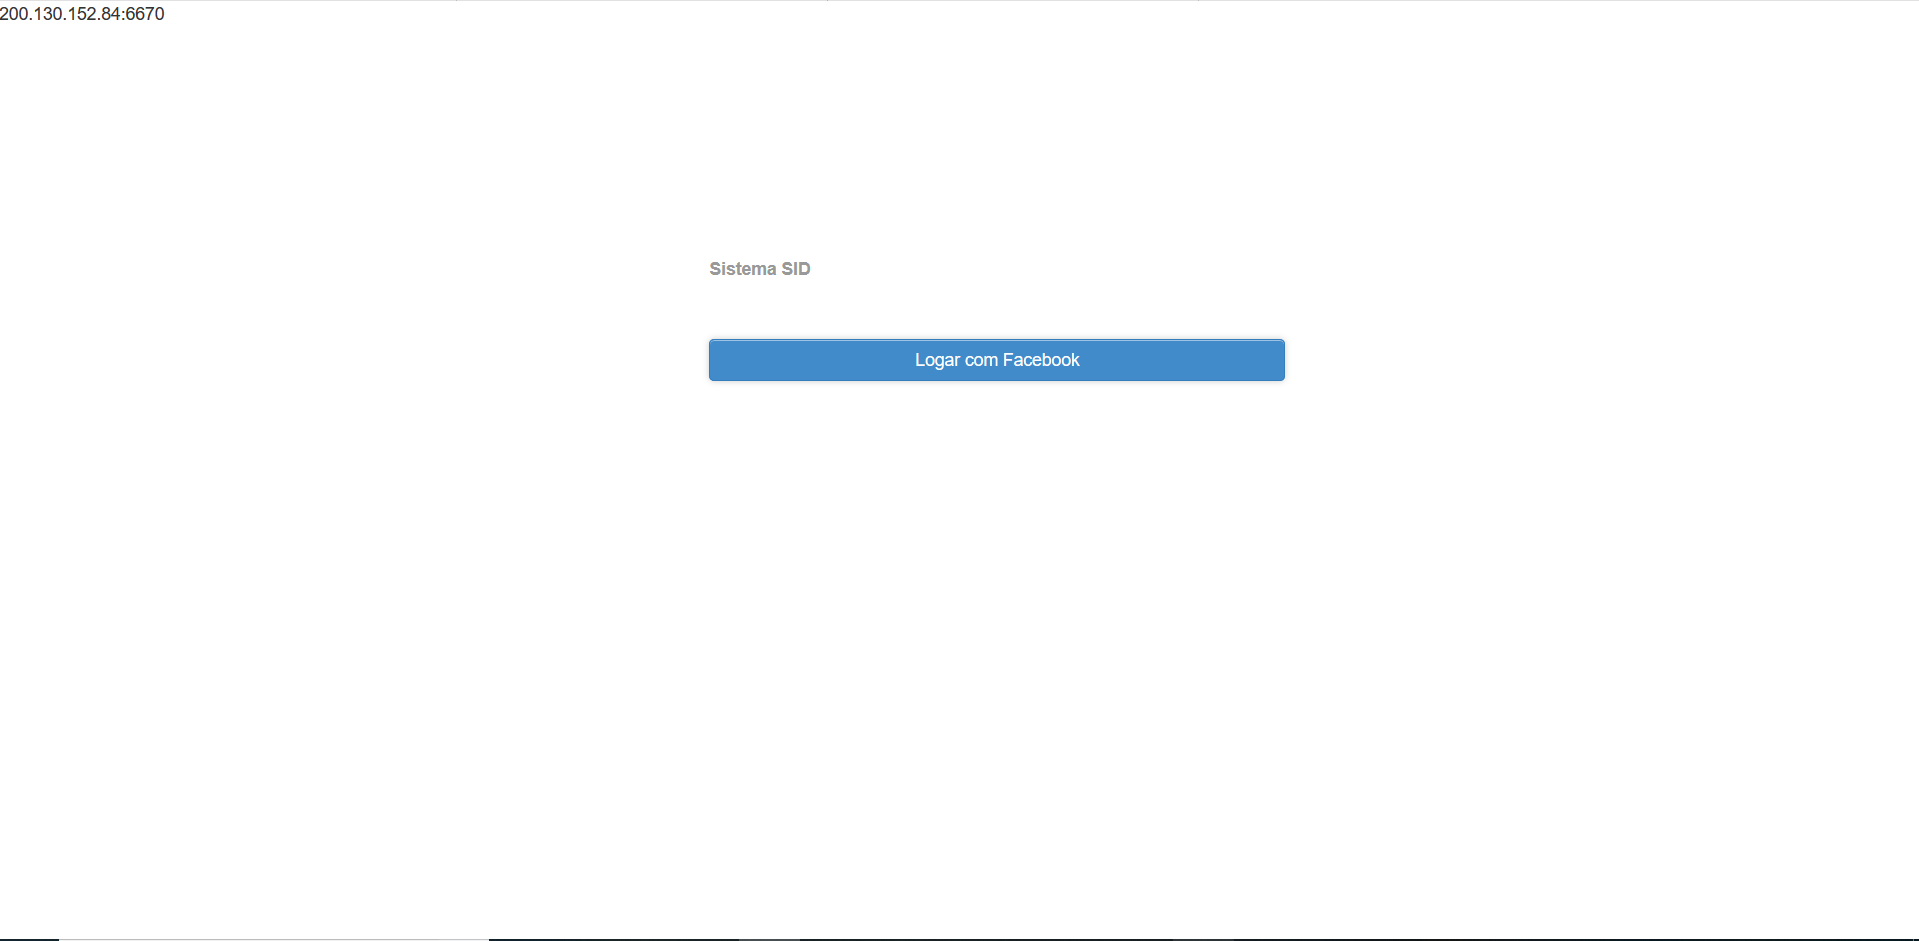
\includegraphics[width=\textwidth]{figuras/telalogar}
                \caption{Tela de login do Administrador}
            \end{figure}
        \item Campos\\
            Não se aplica.
        \item Comandos
            \begin{table}[H]
                \caption{Comandos da tela de logar}
                \resizebox{\textwidth}{!}{%
                \begin{tabular}{|c|c|c|c|c|}
                \hline
Nome & Descrição & Grupo & Requisitos de validade & Requisitos Diversos \\ \hline
Logar com Facebook & Usa a conta do Facebook do usuário para fazer login. & Todos & Autoriza se a conta estiver registrada no banco. & Deve possuir uma conta no Facebook. \\ \hline
                \end{tabular}%
                }
            \end{table}
    \end{itemize}
        
    \subsubsection{Interface do Administrador (Inserir)}
       \begin{itemize}
        \item Leiaute
            \begin{figure}[H]
                \centering
                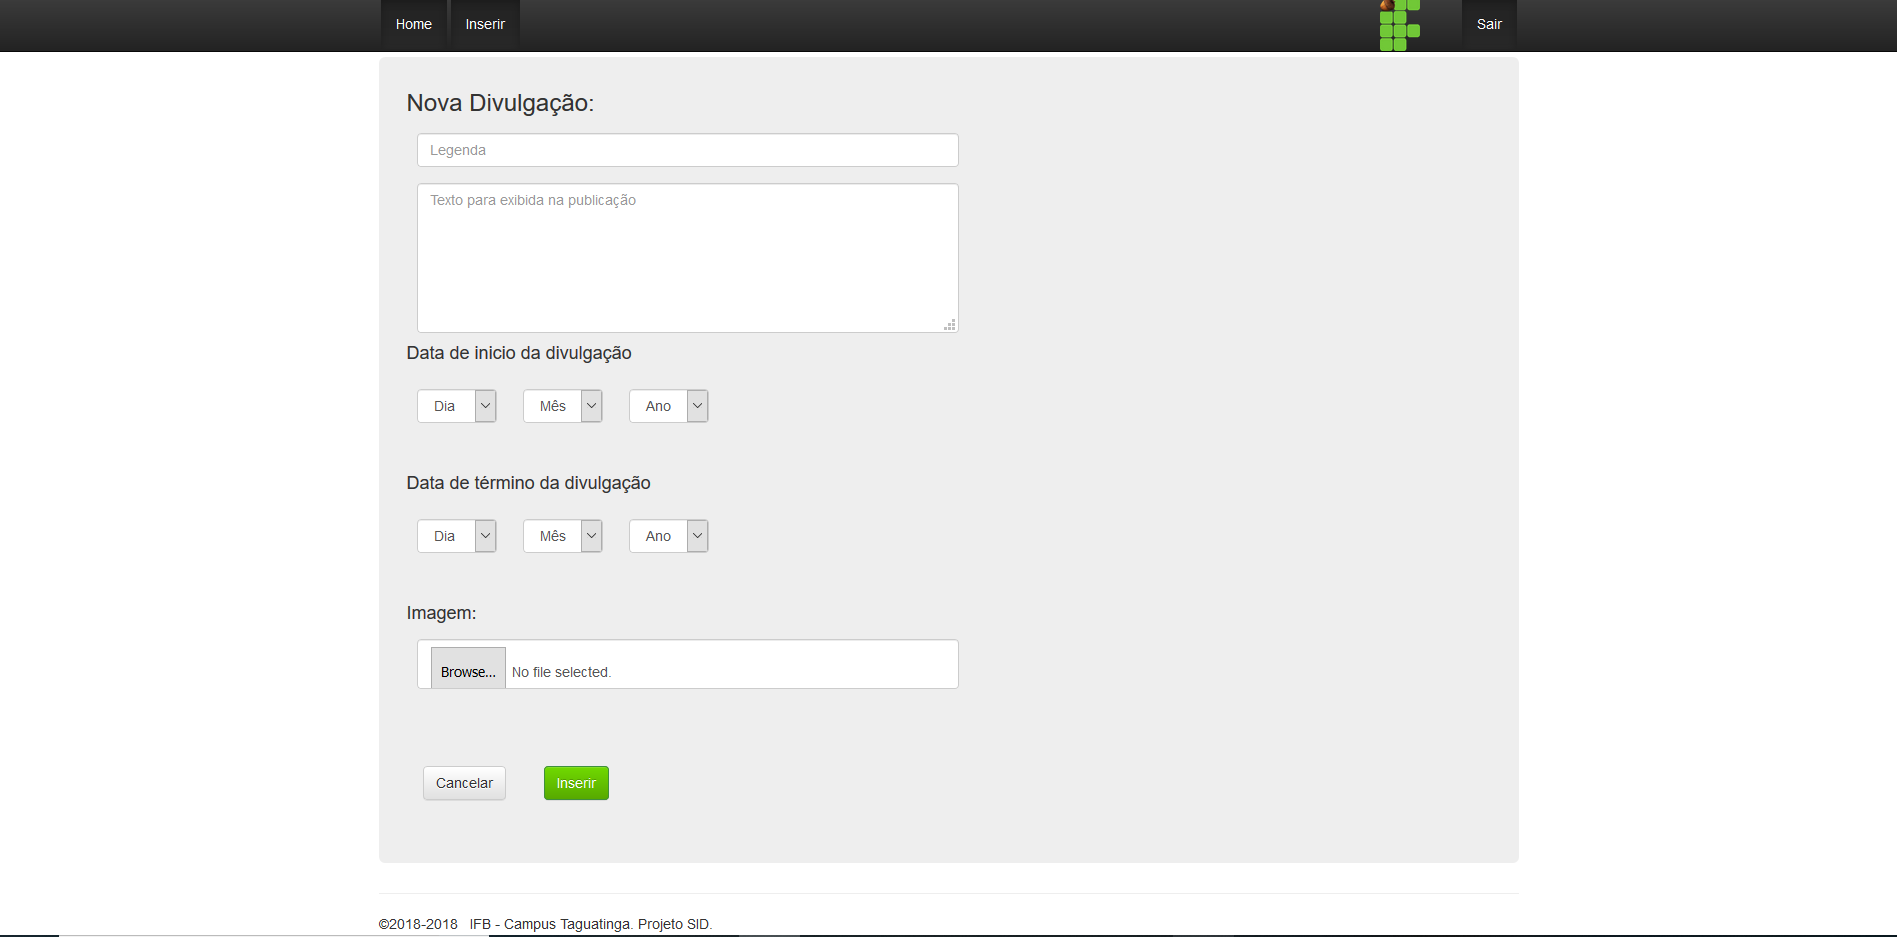
\includegraphics[width=\textwidth]{figuras/telainserir}
                \caption{Tela de inserção de novas publicações}
            \end{figure}
        
        \item Campos
        \begin{table}[H]
            \caption{Campos da tela de inserção}
            \resizebox{\textwidth}{!}{%
                \begin{tabular}{|c|c|c|c|c|c|}
                \hline
Nome & Descrição & Grupo & Requisitos de conteúdo & Requisitos de edição & Requisitos Diversos \\ \hline
Legenda & Legenda que irá ser apresentada no cliente. & Admin & Texto & -- & -- \\ \hline
Texto & Texto da publicação que será postada no Facebook. & Admin & Texto & -- & -- \\ \hline
Data de início & Data em que a publicação começará a ser exibida no cliente. & Admin & Inteiro selecionável entre as opções apresentadas & -- & -- \\ \hline
Data de Término & Data em que a publicação deixará de ser exibida no cliente. & Admin & Inteiro selecionável entre as opções apresentadas & -- & -- \\ \hline
Imagem & Imagem que irá ser apresentada na publicação do Facebook e no Cliente. & Admin & Arquivo do tipo imagem. & -- & A imagem deve ter o formato suportado pelo Facebook \\ \hline
                \end{tabular}%
            }
            \end{table}
        \item Comandos
            \begin{table}[H]
                \caption{Comandos da tela de inserção}
                \resizebox{\textwidth}{!}{%
                \begin{tabular}{|c|c|c|c|c|}
                \hline
Nome & Descrição & Grupo & Requisitos de validade & Requisitos Diversos \\ \hline
Inserir & Insere no banco e no Facebook as informações descritas nos campos. & admin & Todos os campos devem estar preenchidos. & -- \\ \hline
Cancelar & Cancela a inserção dos dados e retorna para a lista de publicações criadas. & admin & -- & -- \\ \hline
                \end{tabular}%
                }
            \end{table}
    \end{itemize}
        
    \subsubsection{Interface do Administrador (Listar)}
        \begin{itemize}
        \item Leiaute
            \begin{figure}[H]
                \centering
                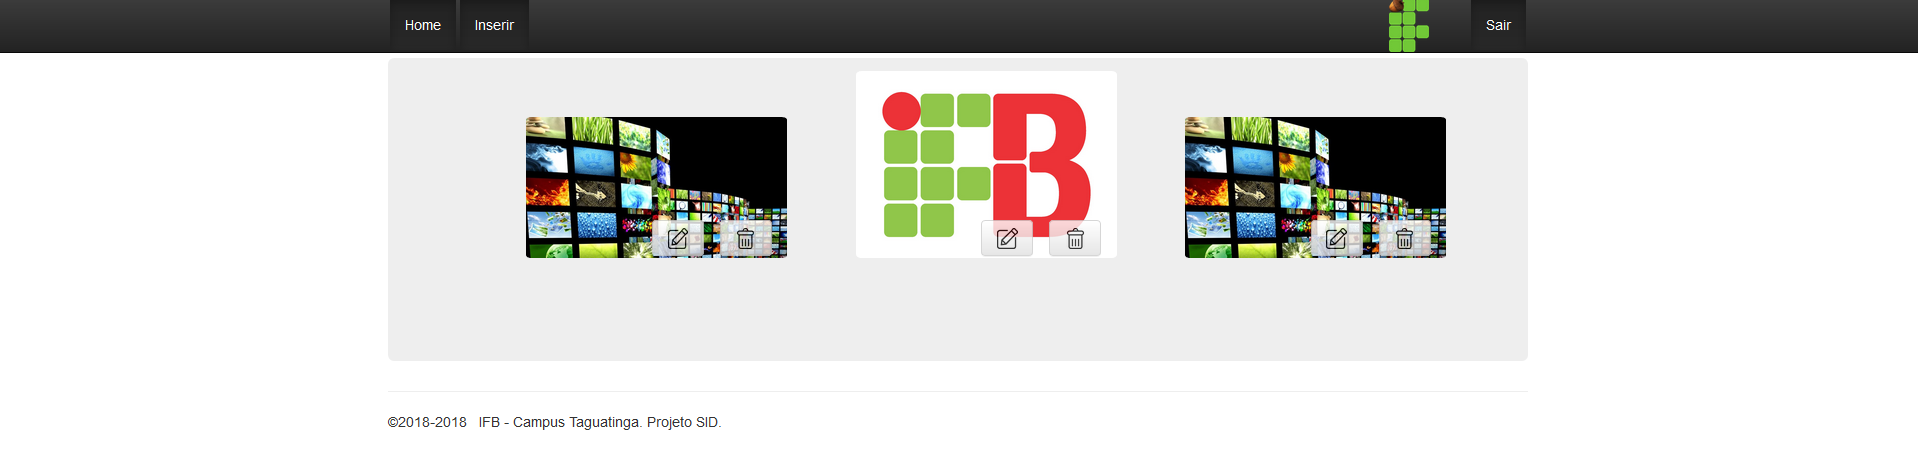
\includegraphics[width=\textwidth]{figuras/telalistar}
                \caption{Tela de listagem das publicações}
            \end{figure}
        \item Campos\\
            Não se aplica.
        \item Comandos
                \begin{table}[H]
                \caption{Comandos da tela de listagem}
                \resizebox{\textwidth}{!}{%
                \begin{tabular}{|c|c|c|c|c|}
                \hline
Nome & Descrição & Grupo & Requisitos de validade & Requisitos Diversos \\ \hline
Detalhar & Clicar sobre a imagem retorna a páginacom  detalhes da publicação. & admin & -- & -- \\ \hline
Editar & O ícone de editar, retorna pagina de edição. & admin & -- & -- \\ \hline
Deletar & O ícone de excluir, exclui a publicação do banco e do Cliente. & admin & -- & -- \\ \hline
                \end{tabular}%
                }
            \end{table}
    \end{itemize}
        
    \subsubsection{Interface do Administrador (Editar)}
        \begin{itemize}
        \item Leiaute
            \begin{figure}[H]
                \centering
                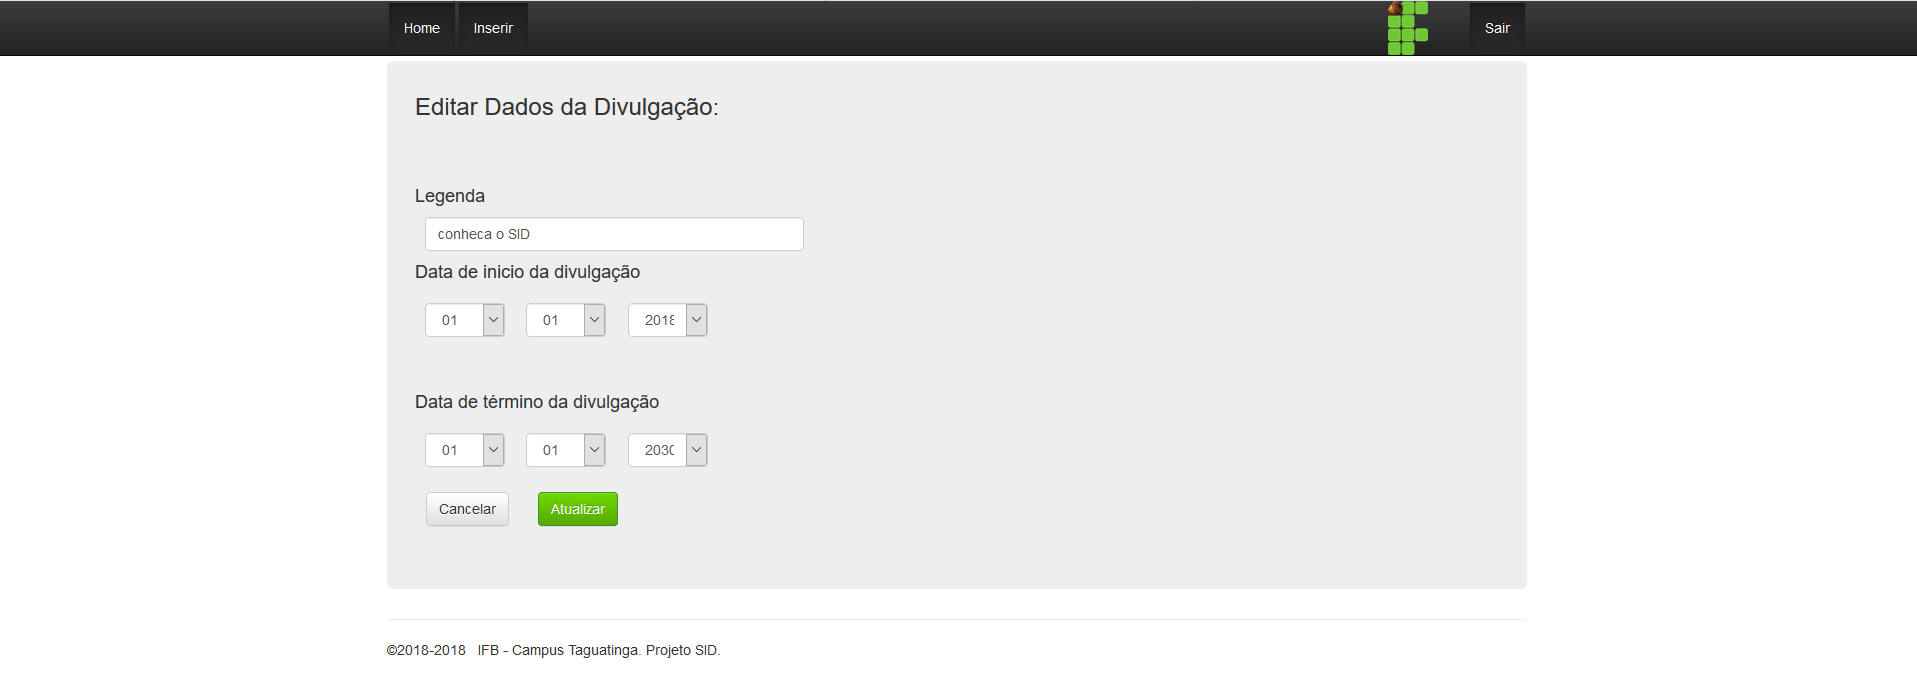
\includegraphics[width=\textwidth]{figuras/telaeditar}
                \caption{Tela de edição das publicações}
            \end{figure}
        \item Campos
\begin{table}[H]
            \caption{Campos da tela de edição}
            \resizebox{\textwidth}{!}{%
                \begin{tabular}{|c|c|c|c|c|c|}
                \hline
Nome & Descrição & Grupo & Requisitos de conteúdo & Requisitos de edição & Requisitos Diversos \\ \hline
Legenda & Legenda que irá ser apresentada no cliente. & Admin & Texto & -- & -- \\ \hline
Data de início & Data em que a publicação começará a ser exibida no cliente. & Admin & Inteiro selecionável entre as opções apresentadas & -- & -- \\ \hline
Data de Término & Data em que a publicação deixará de ser exibida no cliente. & Admin & Inteiro selecionável entre as opções apresentadas & -- & -- \\ \hline
                \end{tabular}%
            }
            \end{table}
        \item Comandos
            \begin{table}[H]
                \caption{Comandos da tela de edição}
                \resizebox{\textwidth}{!}{%
                \begin{tabular}{|c|c|c|c|c|}
                \hline
Nome & Descrição & Grupo & Requisitos de validade & Requisitos Diversos \\ \hline
Atualizar & Realiza a atualização no banco com os novos dados & admin & Todos os campos devem estar preenchidos & -- \\ \hline
Cancelar & Cancela as alterações e retorna a página de listagem & admin & -- & -- \\ \hline
                \end{tabular}%
                }
            \end{table}
    \end{itemize}
        
    \subsubsection{Interface do Administrador (Detalhar)}
        \begin{itemize}
        \item Leiaute
            \begin{figure}[H]
                \centering
                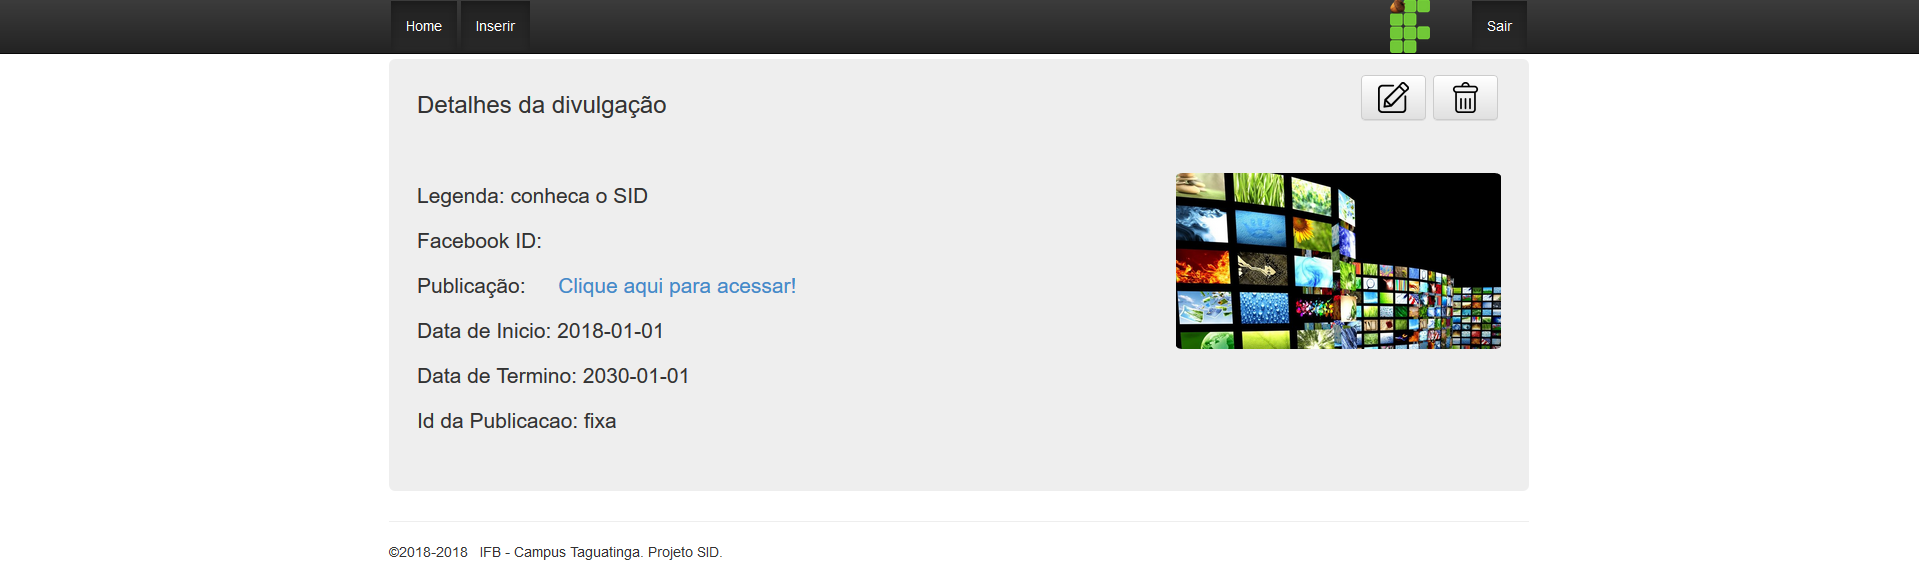
\includegraphics[width=\textwidth]{figuras/teladetalhar}
                \caption{Tela de detalhamento das publicações}
            \end{figure}
        \item Campos\\
            Não se aplica.
        \item Comandos
            \begin{table}[H]
                \caption{Comandos da tela de detalhamento}
                \resizebox{\textwidth}{!}{%
                \begin{tabular}{|c|c|c|c|c|}
                \hline
Nome & Descrição & Grupo & Requisitos de validade & Requisitos Diversos \\ \hline
Clique Aqui & Acessa aolink da publicação no Facebook. & admin & -- & -- \\ \hline
Editar & O ícone de editar, retorna pagina de edição. & admin & -- & -- \\ \hline
Deletar & O ícone de excluir, exclui a publicação do banco e do Cliente. & admin & -- & -- \\ \hline
                \end{tabular}%
                }
            \end{table}
    \end{itemize}
        
    \subsubsection{Interface Cliente}
        \begin{itemize}
        \item Leiaute
            \begin{figure}[H]
                \centering
                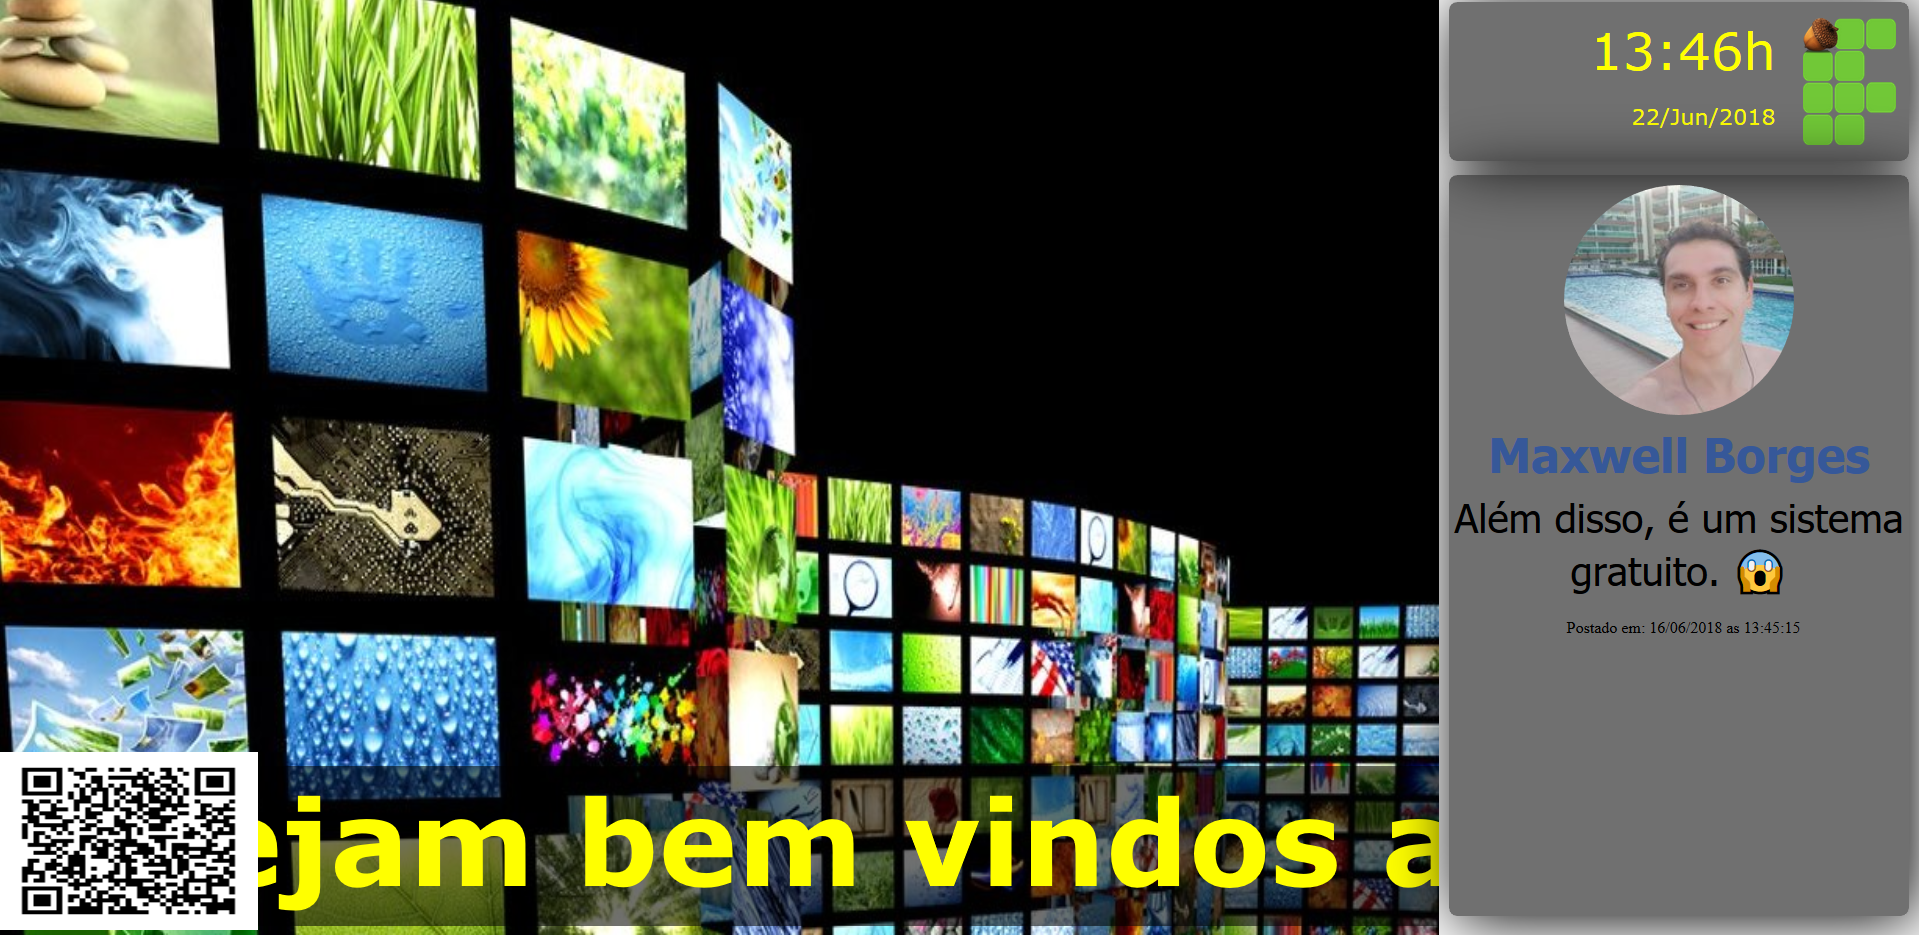
\includegraphics[width=\textwidth]{figuras/telacliente}
                \caption{Tela do cliente}
            \end{figure}
        \item Campos\\
            Não se aplica.
        \item Comandos\\
            Não se aplica.
        \end{itemize}
\clearpage

\section{Diagramas}
\label{diagramas}
\subsection{Diagramas de casos de uso}
\begin{figure}[H]
    \centering
    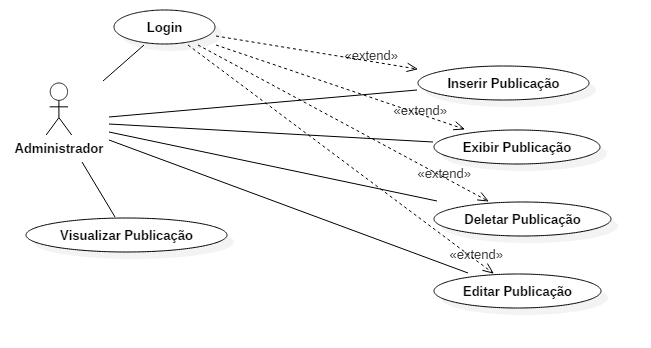
\includegraphics[width=\textwidth]{figuras/casosDeUsoADM}
    \caption{Diagrama de casos de uso do módulo administrador}
\end{figure}

\begin{figure}[H]
    \centering
    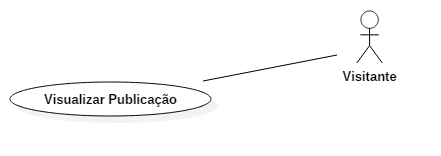
\includegraphics[width=\textwidth]{figuras/CasosDeUsoCliente}
    \caption{Diagrama de casos de uso do módulo cliente}
\end{figure}

\begin{figure}
    \centering
    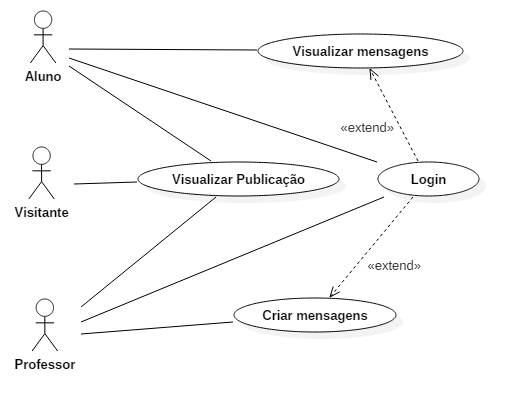
\includegraphics[width=\textwidth]{figuras/CasosDeUsoMobile}
    \caption{Diagrama de casos de uso do aplicativo móvel}
\end{figure}

\subsection{Diagramas de classe}
\begin{figure}[H]
    \centering
    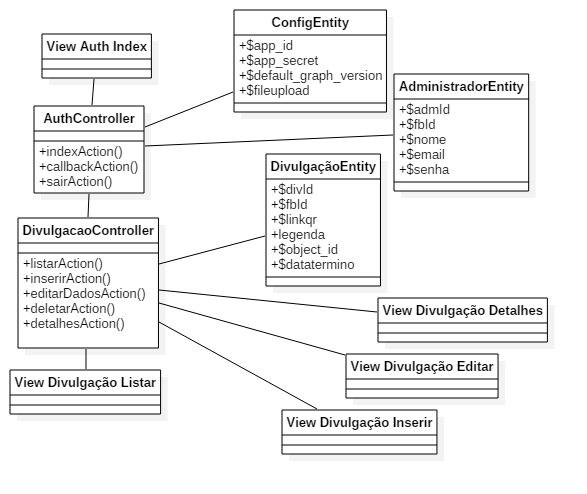
\includegraphics[width=\textwidth]{figuras/diagramaclasseADM}
    \caption{Diagrama de classes do módulo administrador}
\end{figure}

\begin{figure}[H]
    \centering
    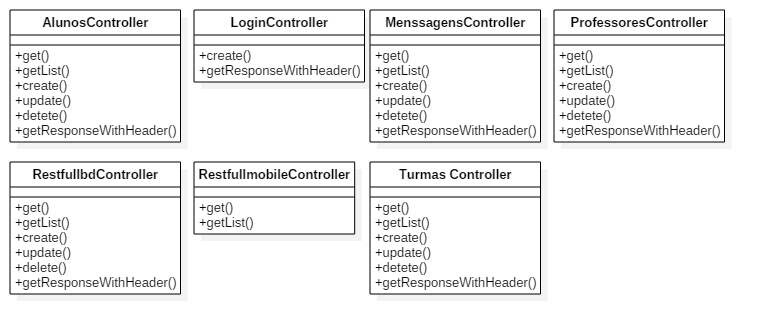
\includegraphics[width=\textwidth]{figuras/diagramaclasseAPI}
    \caption{Diagrama de classes do submódulo API}
\end{figure}

\begin{figure}[H]
    \centering
    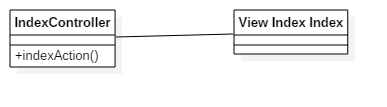
\includegraphics[width=\textwidth]{figuras/diagramaclasseCLIENTE}
    \caption{Diagrama de classes do módulo Cliente}
\end{figure}

\subsection{Diagramas entidade--relacionamento}
\begin{figure}[H]
    \centering
    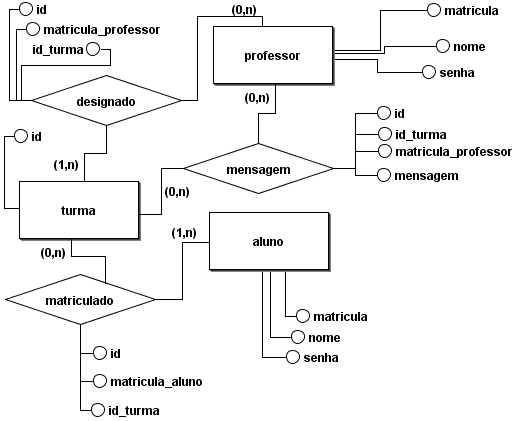
\includegraphics[width=\textwidth]{figuras/entidaderelacionamentomobile}
    \caption{Diagrama entidade--relacionamento do aplicativo móvel (API fictícia)}
\end{figure}

\begin{figure}[H]
    \centering
    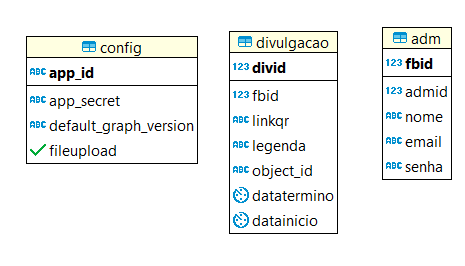
\includegraphics[width=\textwidth]{figuras/entidaderelacionamento}
    \caption{Diagrama entidade--relacionamento do \textit{web}}
\end{figure}

\subsection{Diagramas de sequência}
\begin{figure}[H]
    \centering
    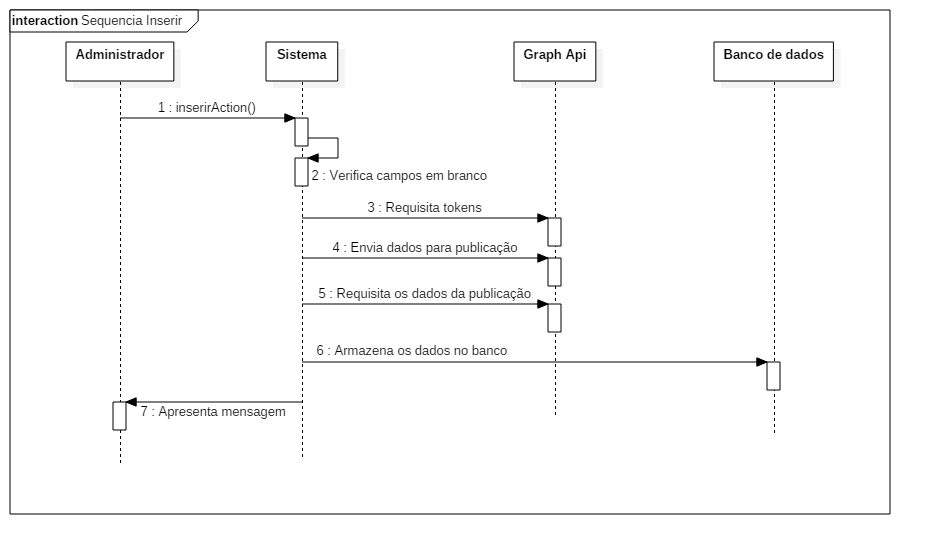
\includegraphics[width=\textwidth]{figuras/sequenciainserir}
    \caption{Diagrama de sequência para inserir}
\end{figure}

\begin{figure}[H]
    \centering
    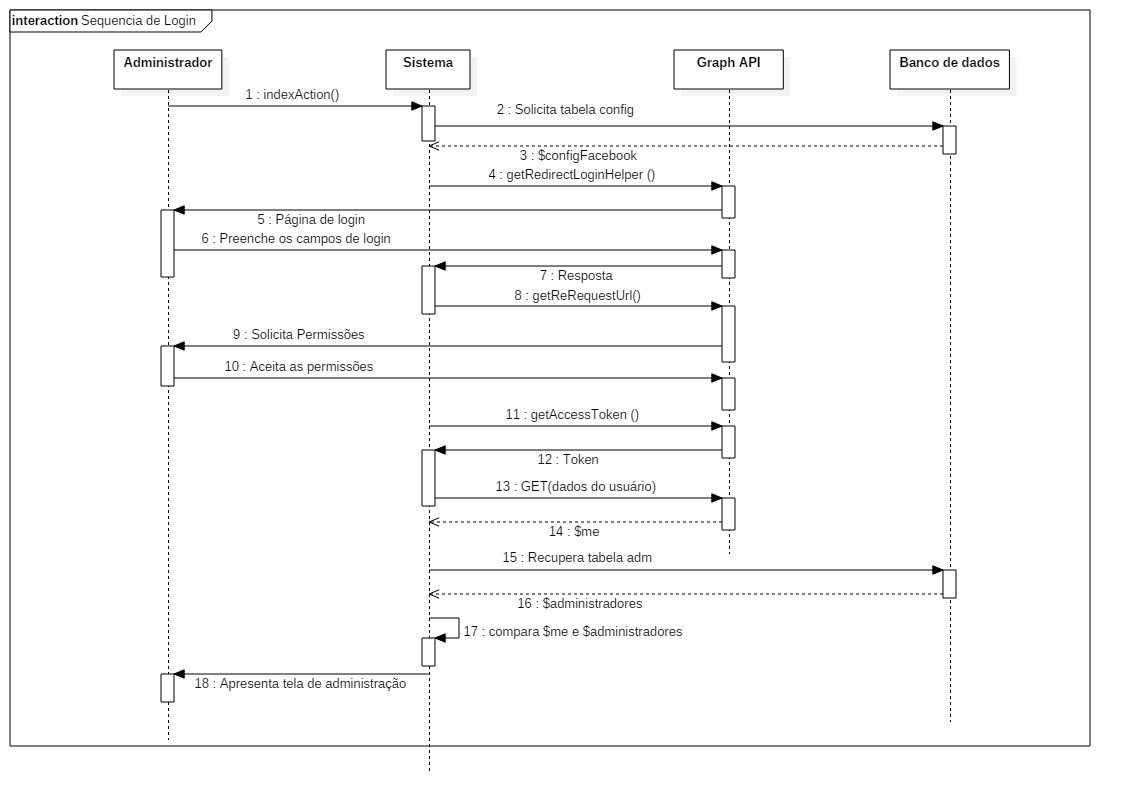
\includegraphics[width=\textwidth]{figuras/sequencialogin}
    \caption{Diagrama de sequência para login}
\end{figure}

\begin{figure}[H]
    \centering
    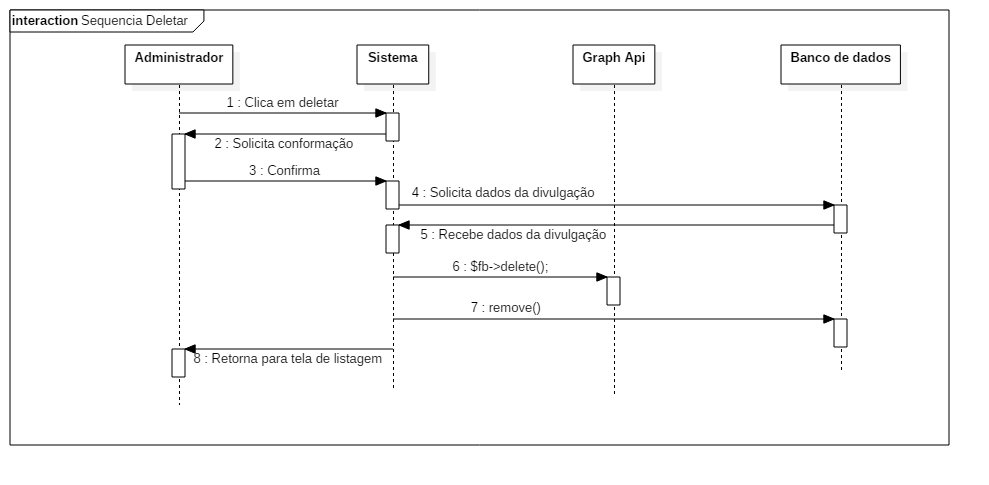
\includegraphics[width=\textwidth]{figuras/sequenciaDeletar}
    \caption{Diagrama de sequência para deletar}
\end{figure}

\begin{figure}[H]
    \centering
    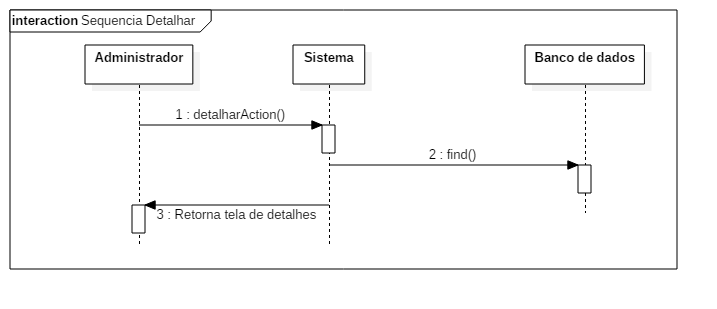
\includegraphics[width=\textwidth]{figuras/sequenciaDetalhar}
    \caption{Diagrama de sequência para detalhar}
\end{figure}

\begin{figure}[H]
    \centering
    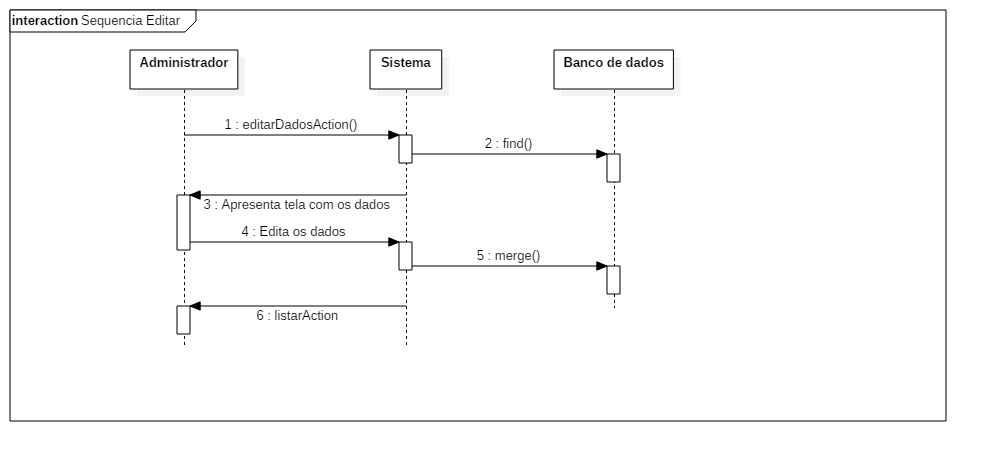
\includegraphics[width=\textwidth]{figuras/sequenciaEditar}
    \caption{Diagrama de sequência para editar}
\end{figure}

\begin{figure}[H]
    \centering
    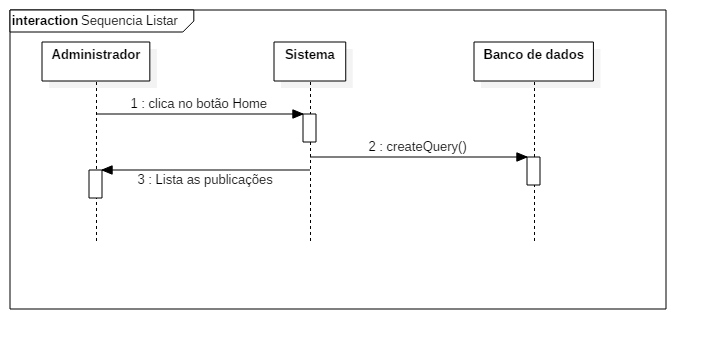
\includegraphics[width=\textwidth]{figuras/sequenciaListar}
    \caption{Diagrama de sequência para listar}
\end{figure}
\clearpage

\section{Artefatos}
\label{artefatos}
\begin{table}[H]
\fontsize{8}{12}\selectfont
\caption{Requisitos de usuário}
\resizebox{\textwidth}{!}{%
\begin{tabular}{p{0.7cm}p{8cm}}
{[}RU01{]} & O sistema deverá permitir login dos administradores através do Facebook ou usando e--mail e senha do usuário cadastrados, autorizando que acessem ao sistema e nele realize as funções permitidas. \\
{[}RU02{]} & O sistema deverá permitir que o usuário devidamente cadastrado consiga criar publicações. \\
{[}RU03{]} & O sistema deverá permitir que o usuário devidamente cadastrado consiga editar as publicações que foram criadas. \\
{[}RU04{]} & O sistema deverá permitir que o usuário devidamente cadastrado consiga excluir uma ou mais publicações criadas. \\
{[}RU05{]} & O sistema deverá confirmar se o usuário deseja excluir uma publicação. \\
{[}RU06{]} & O sistema deverá listar todas as publicações criadas. \\
{[}RU07{]} & O sistema deverá armazenar todas as informações que forem inseridas para que possam serem feitas as edições, listagens e exclusões. \\
{[}RU08{]} & O sistema deverá possuir uma página de acesso público. \\
{[}RU09{]} & O sistema deverá apresentar apenas as publicações e comentários autorizados. \\
{[}RU10{]} & O sistema deverá possuir internet conectada. \\
{[}RU11{]} & O sistema deverá funcionar nos navegadores de internet dos sistemas operacionais Linux, Windows.
\end{tabular}%
}
\end{table}

\begin{figure}
    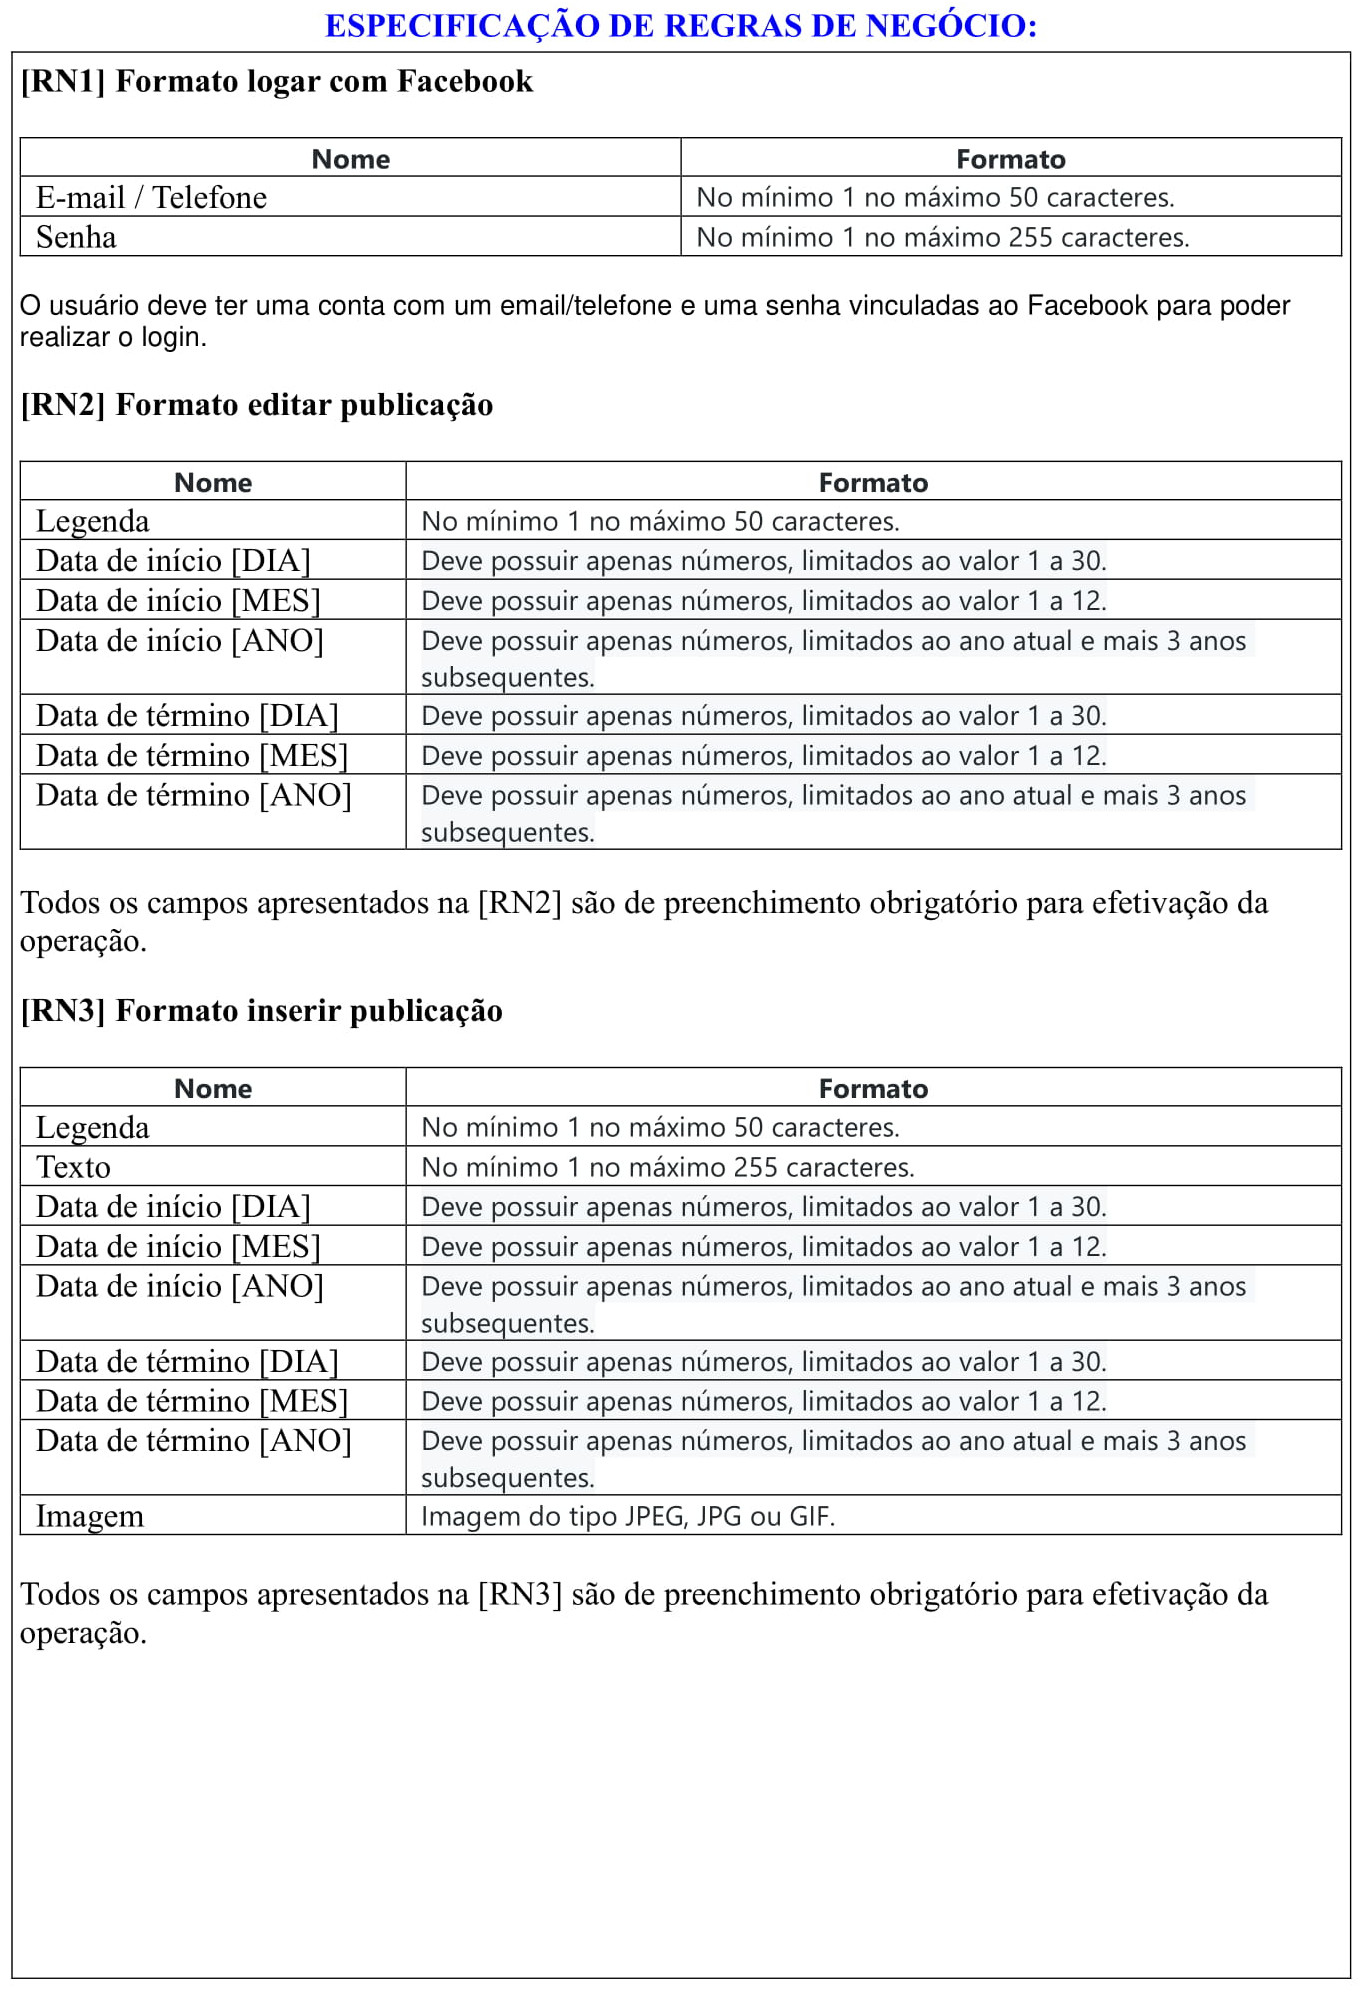
\includegraphics[width=\textwidth]{documentacao/ModeloArtefatos-01.jpg}
\end{figure}

\begin{figure}
    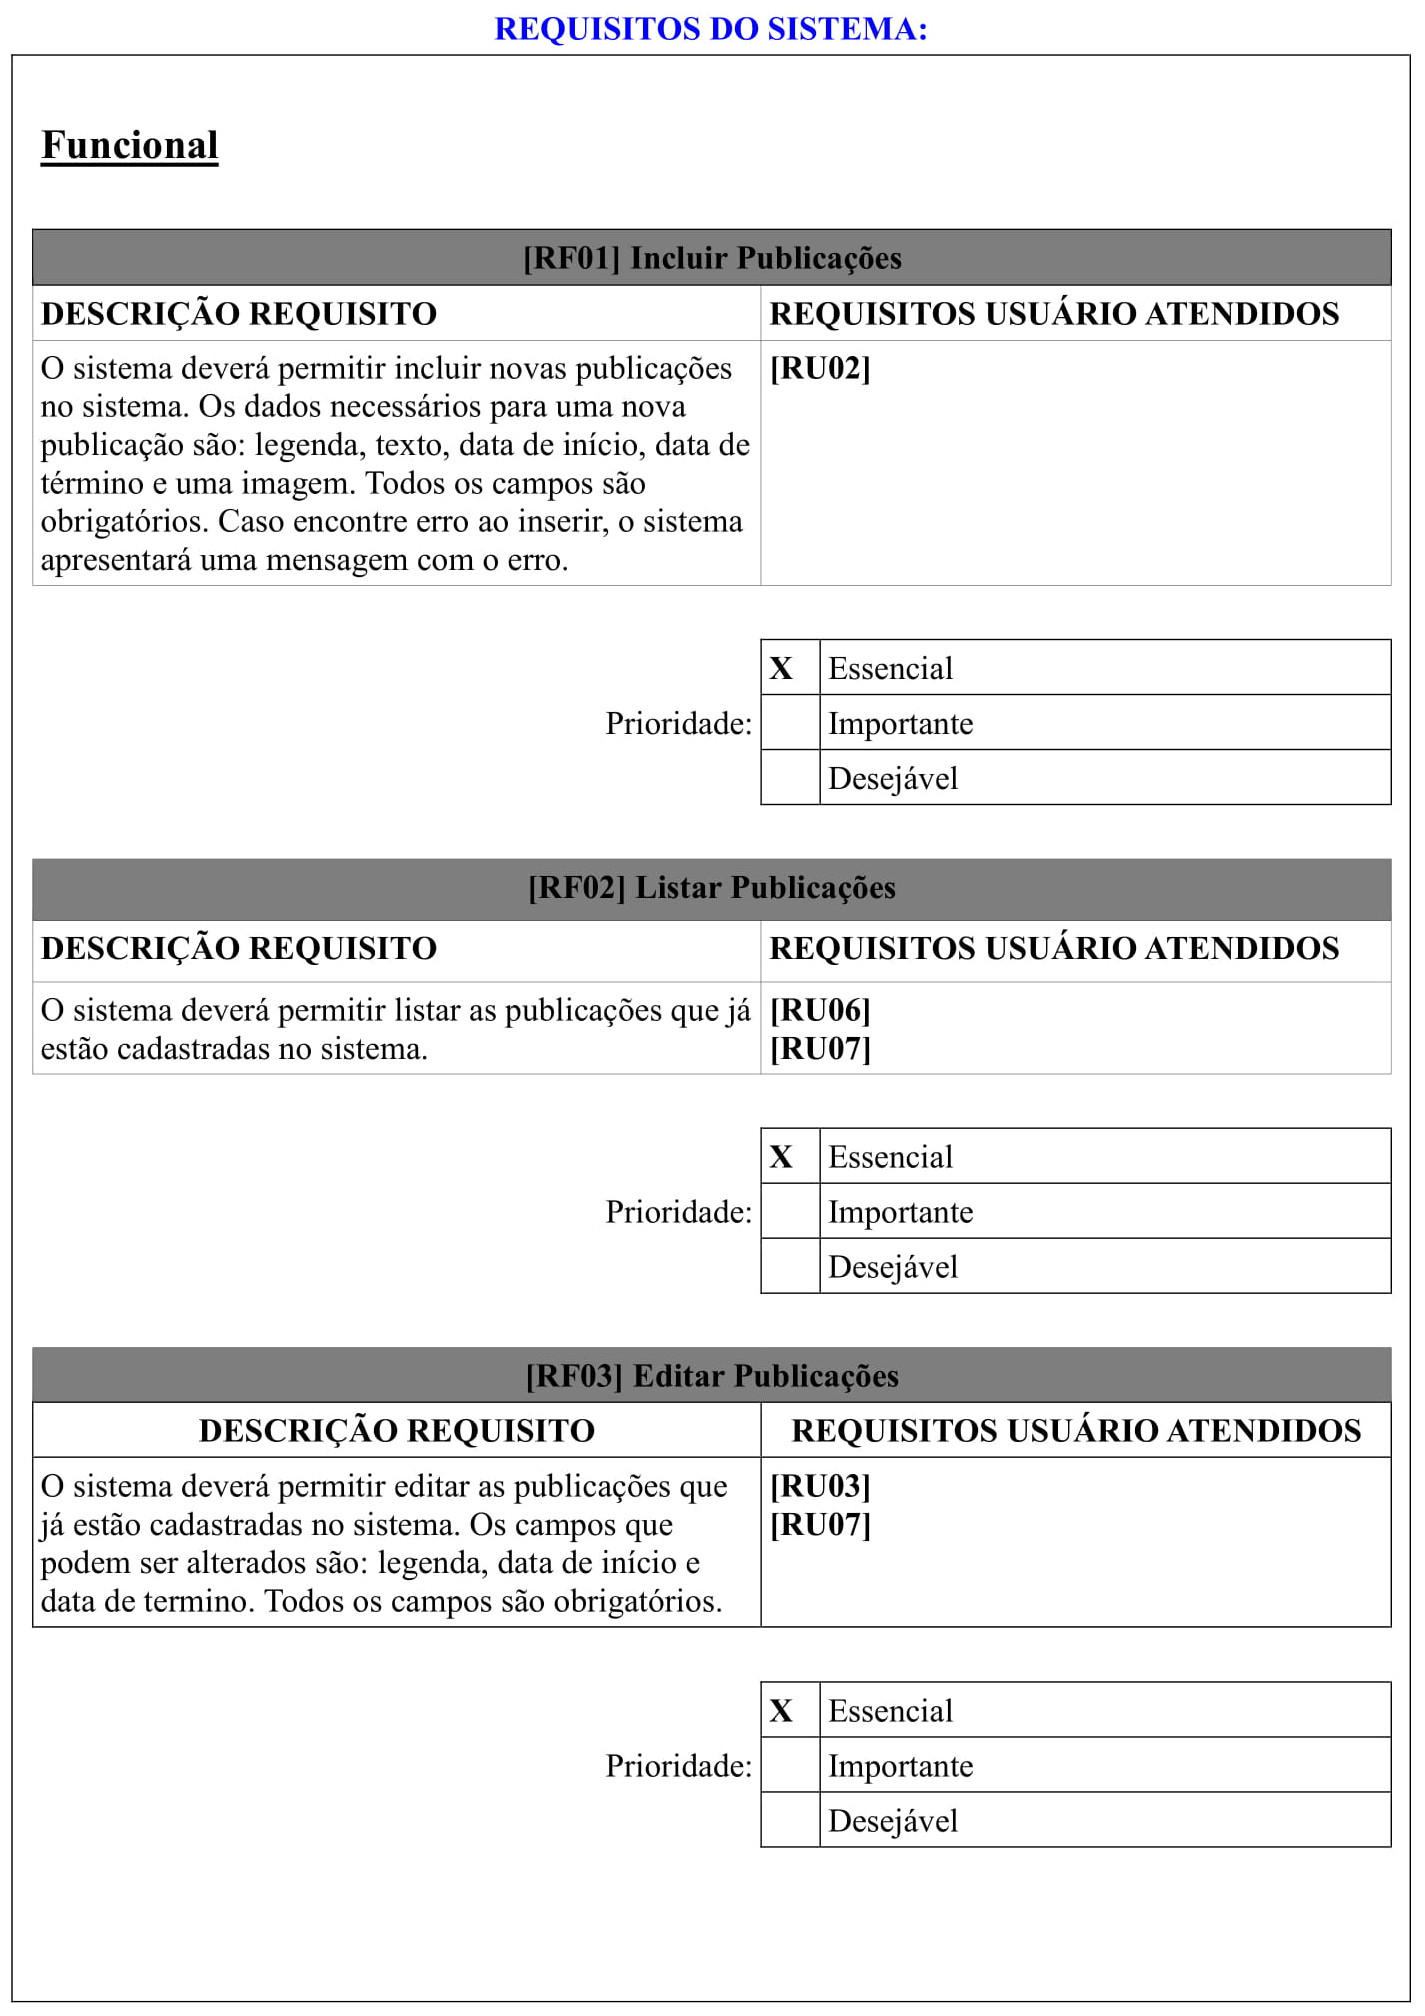
\includegraphics[width=\textwidth]{documentacao/ModeloArtefatos-02.jpg}
\end{figure}

\begin{figure}
    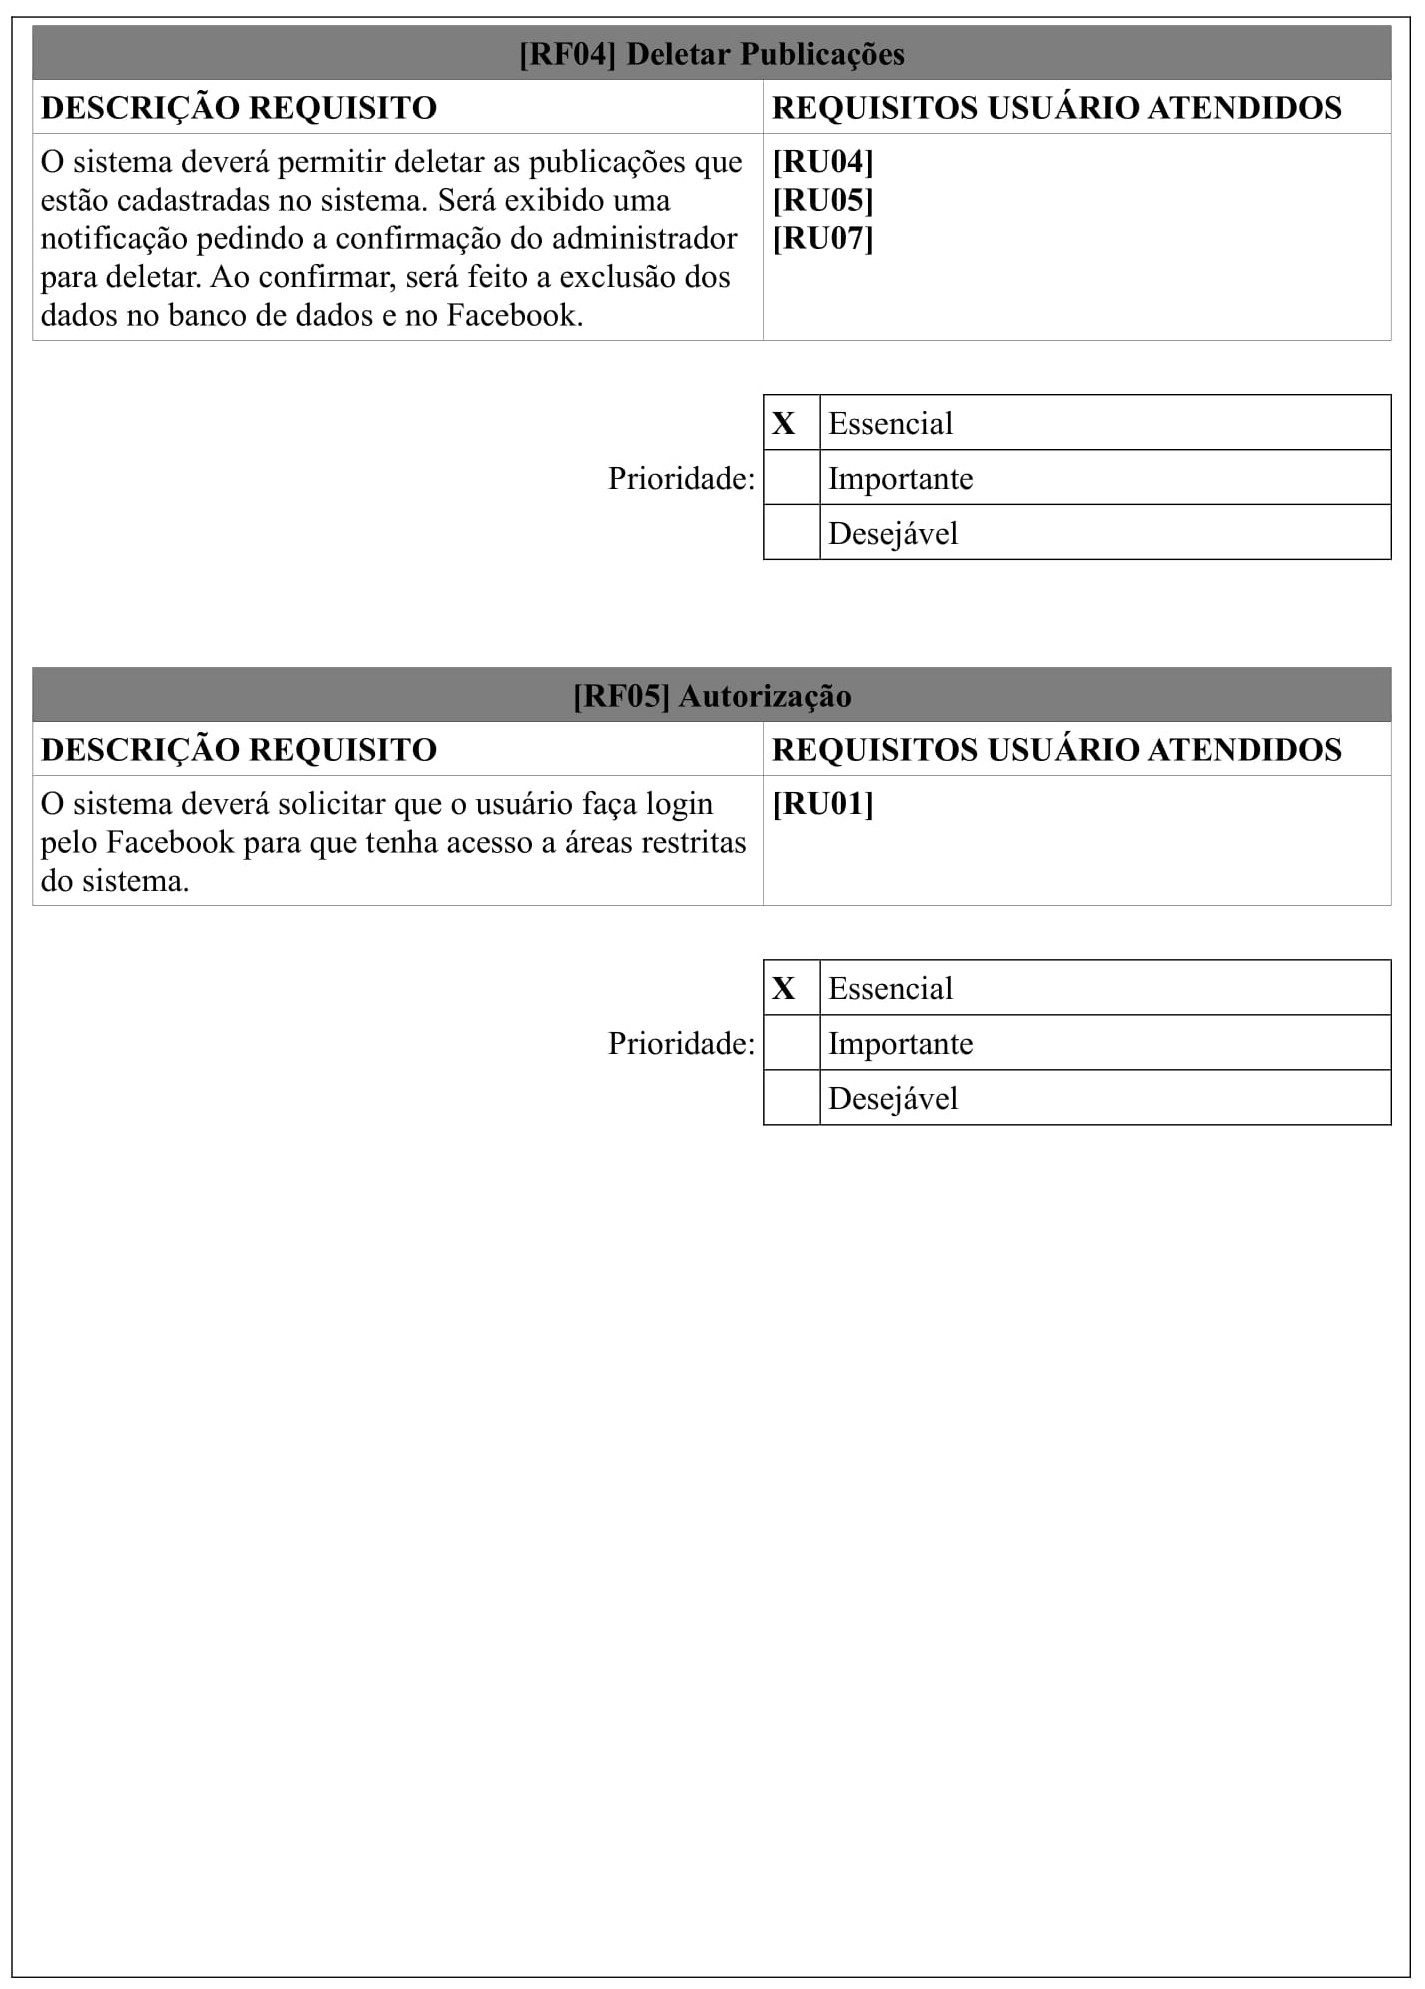
\includegraphics[width=\textwidth]{documentacao/ModeloArtefatos-03.jpg}
\end{figure}

\begin{figure}
    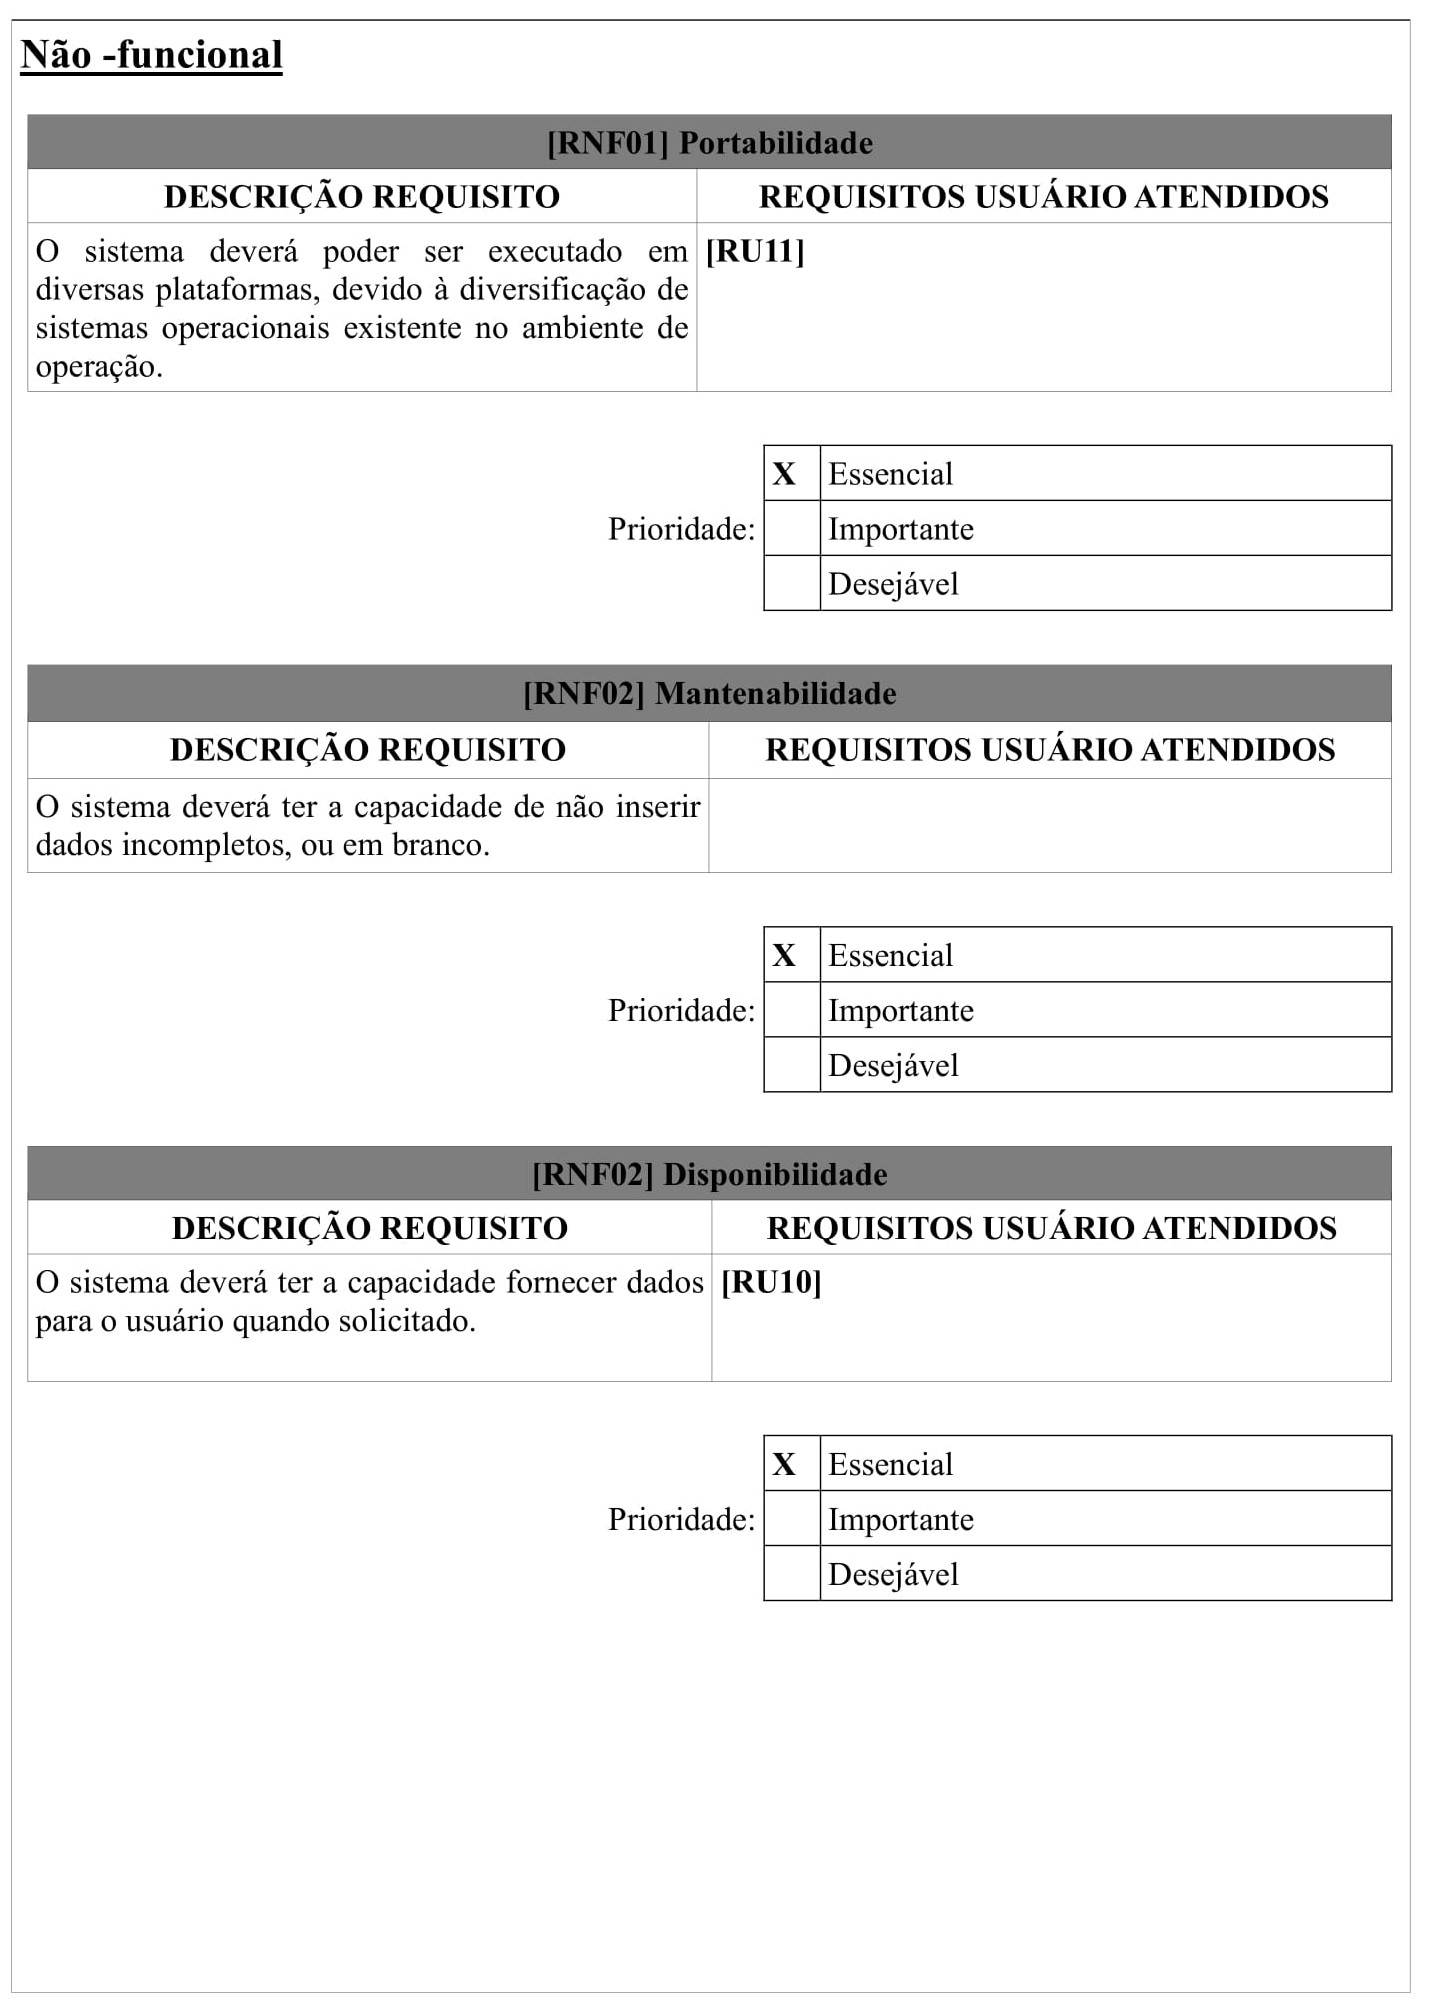
\includegraphics[width=\textwidth]{documentacao/ModeloArtefatos-04.jpg}
\end{figure}

\begin{figure}
    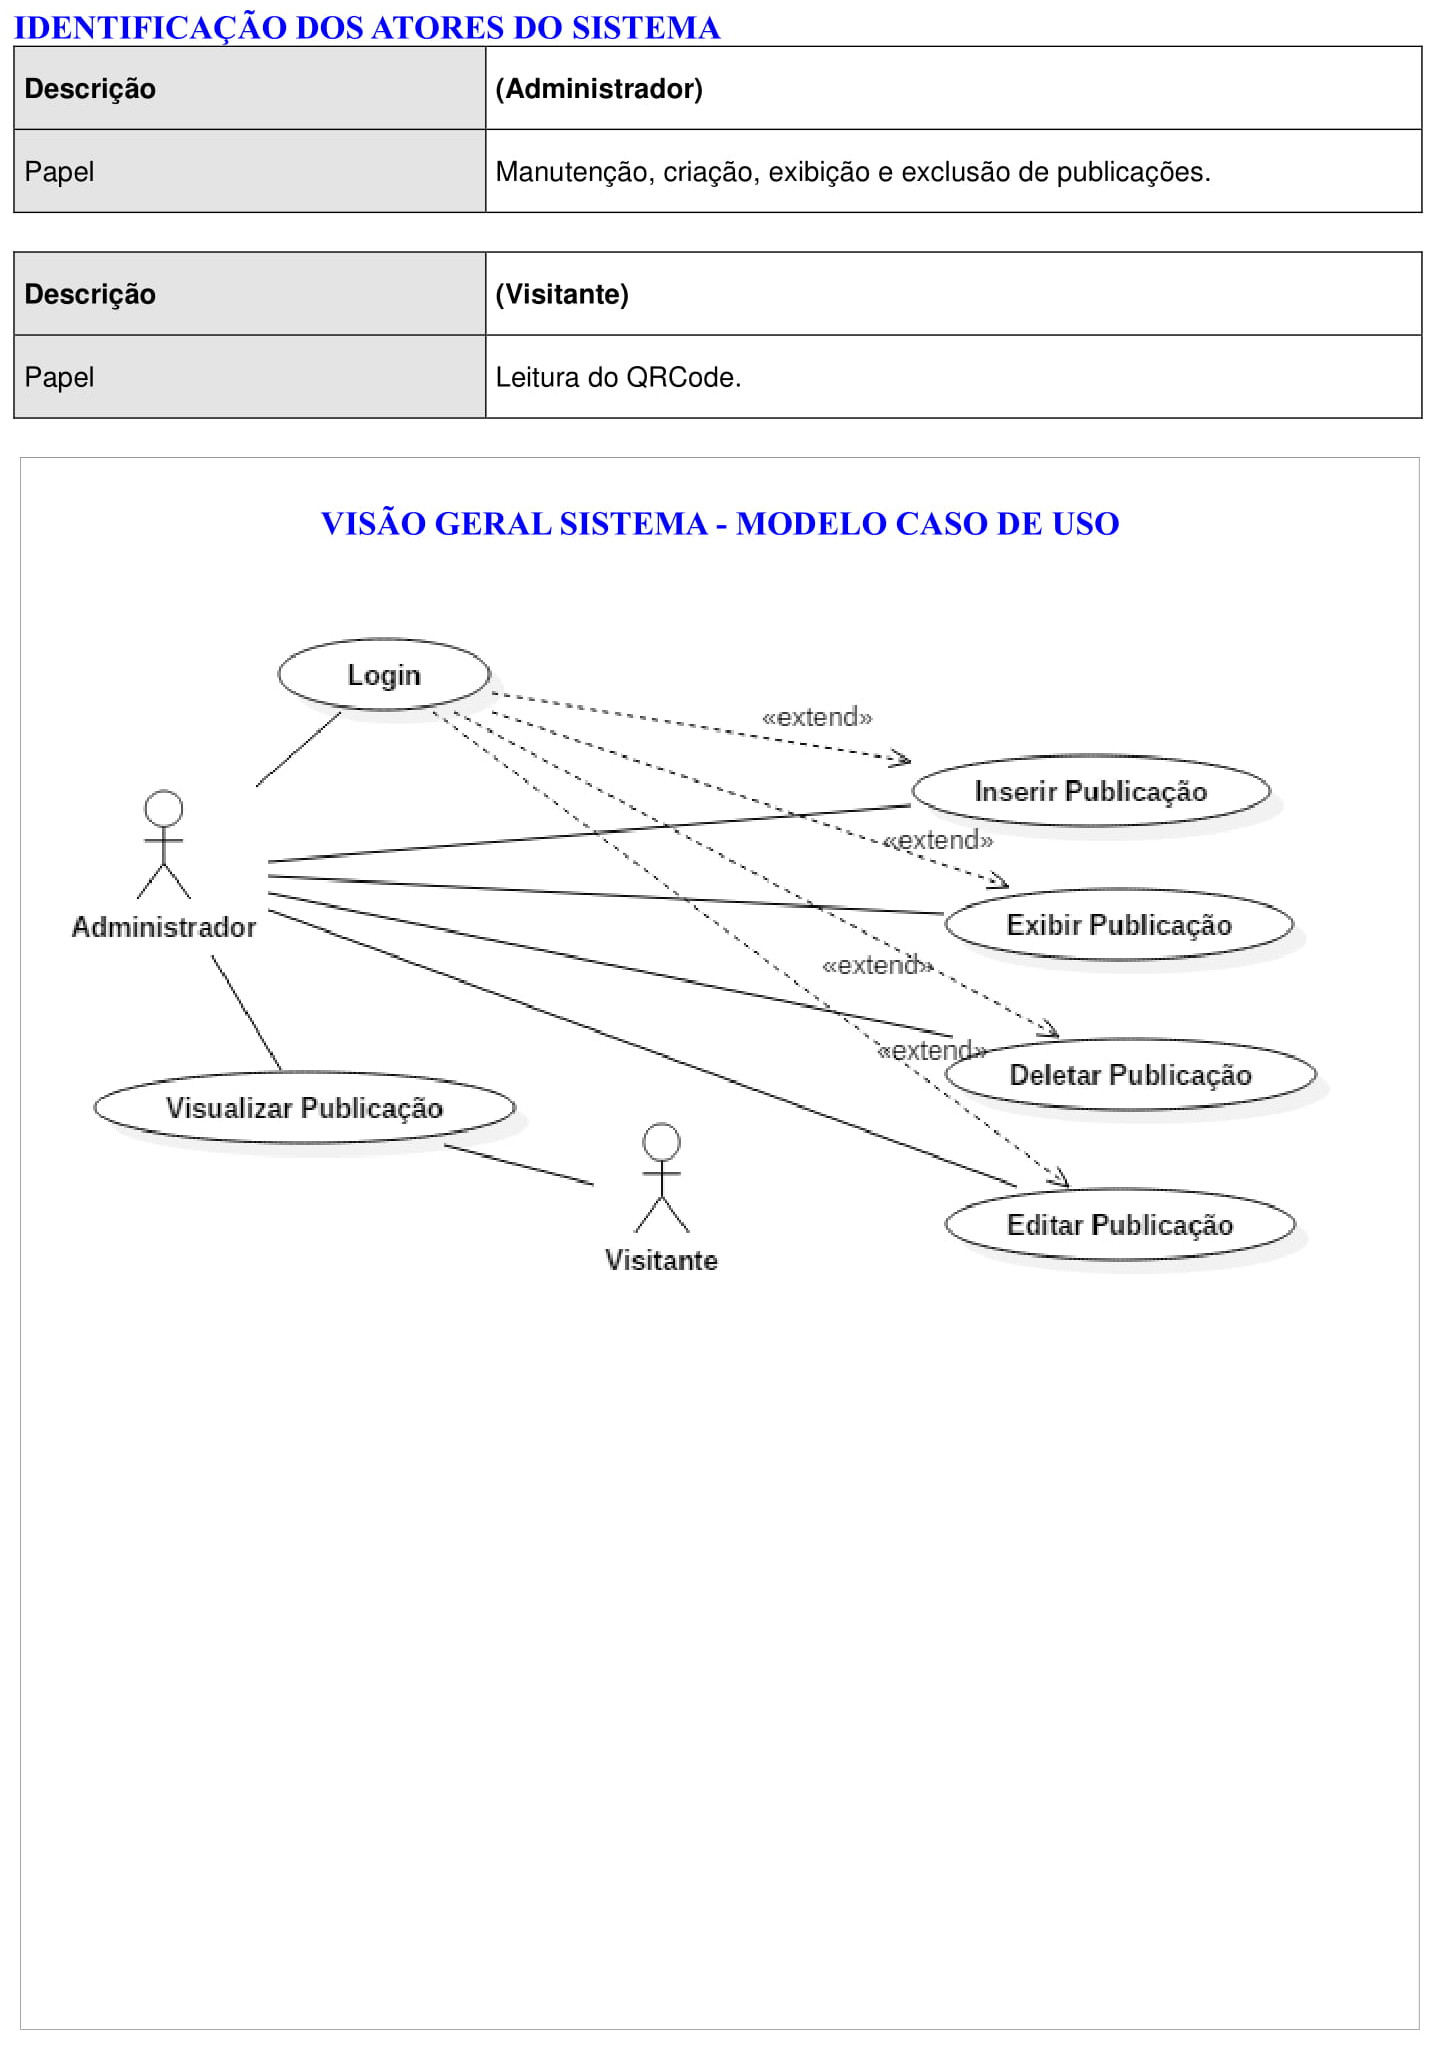
\includegraphics[width=\textwidth]{documentacao/ModeloArtefatos-05.jpg}
\end{figure}

\begin{figure}
    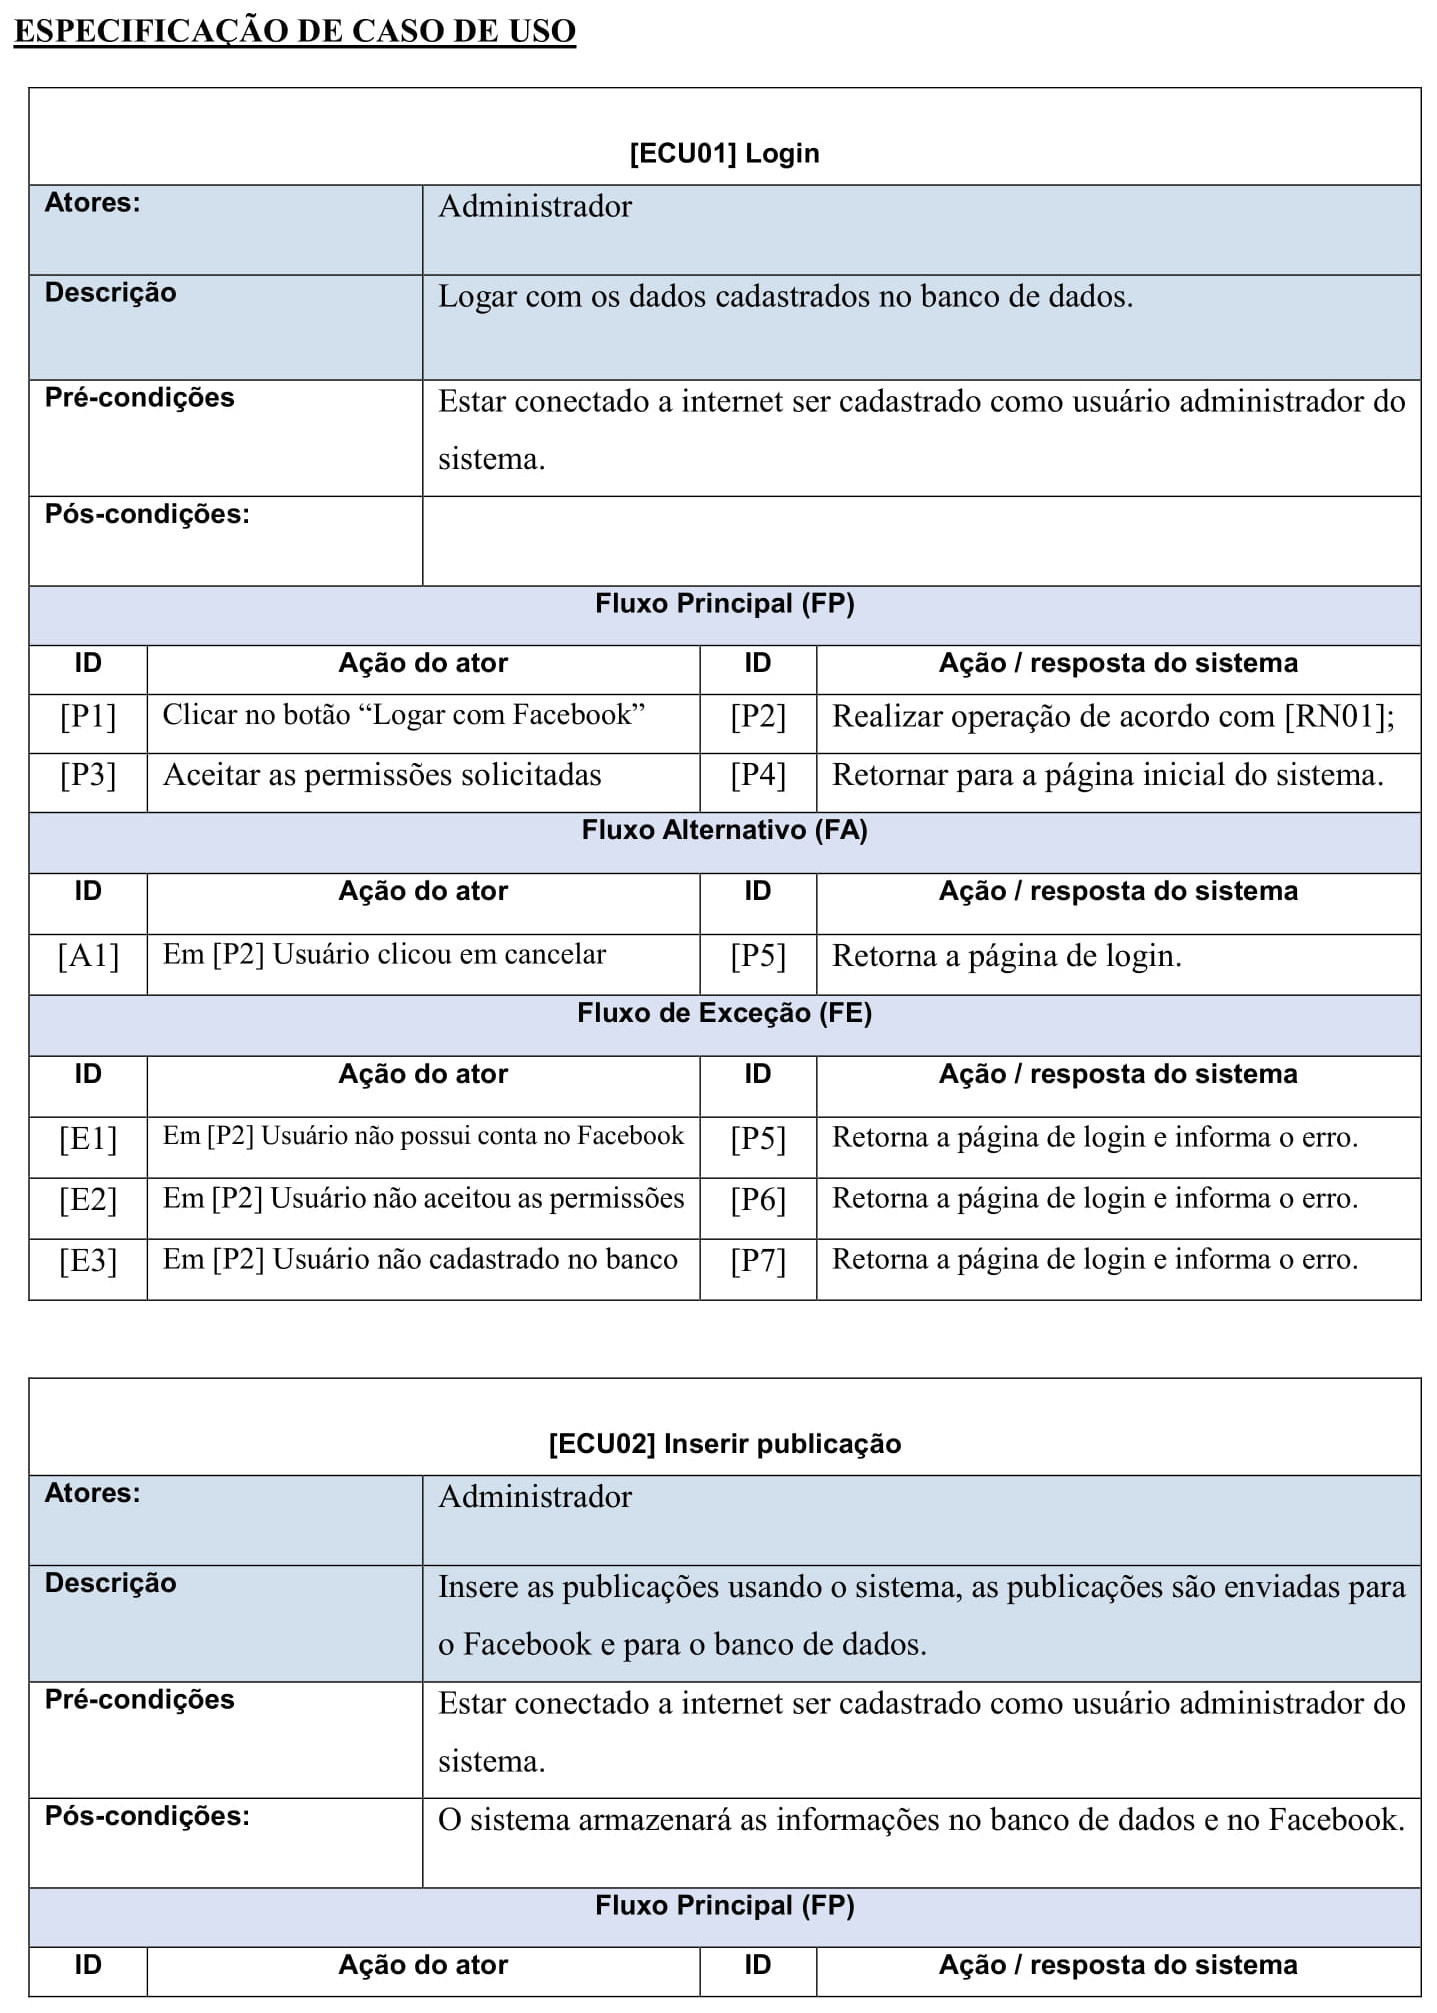
\includegraphics[width=\textwidth]{documentacao/ModeloArtefatos-06.jpg}
\end{figure}

\begin{figure}
    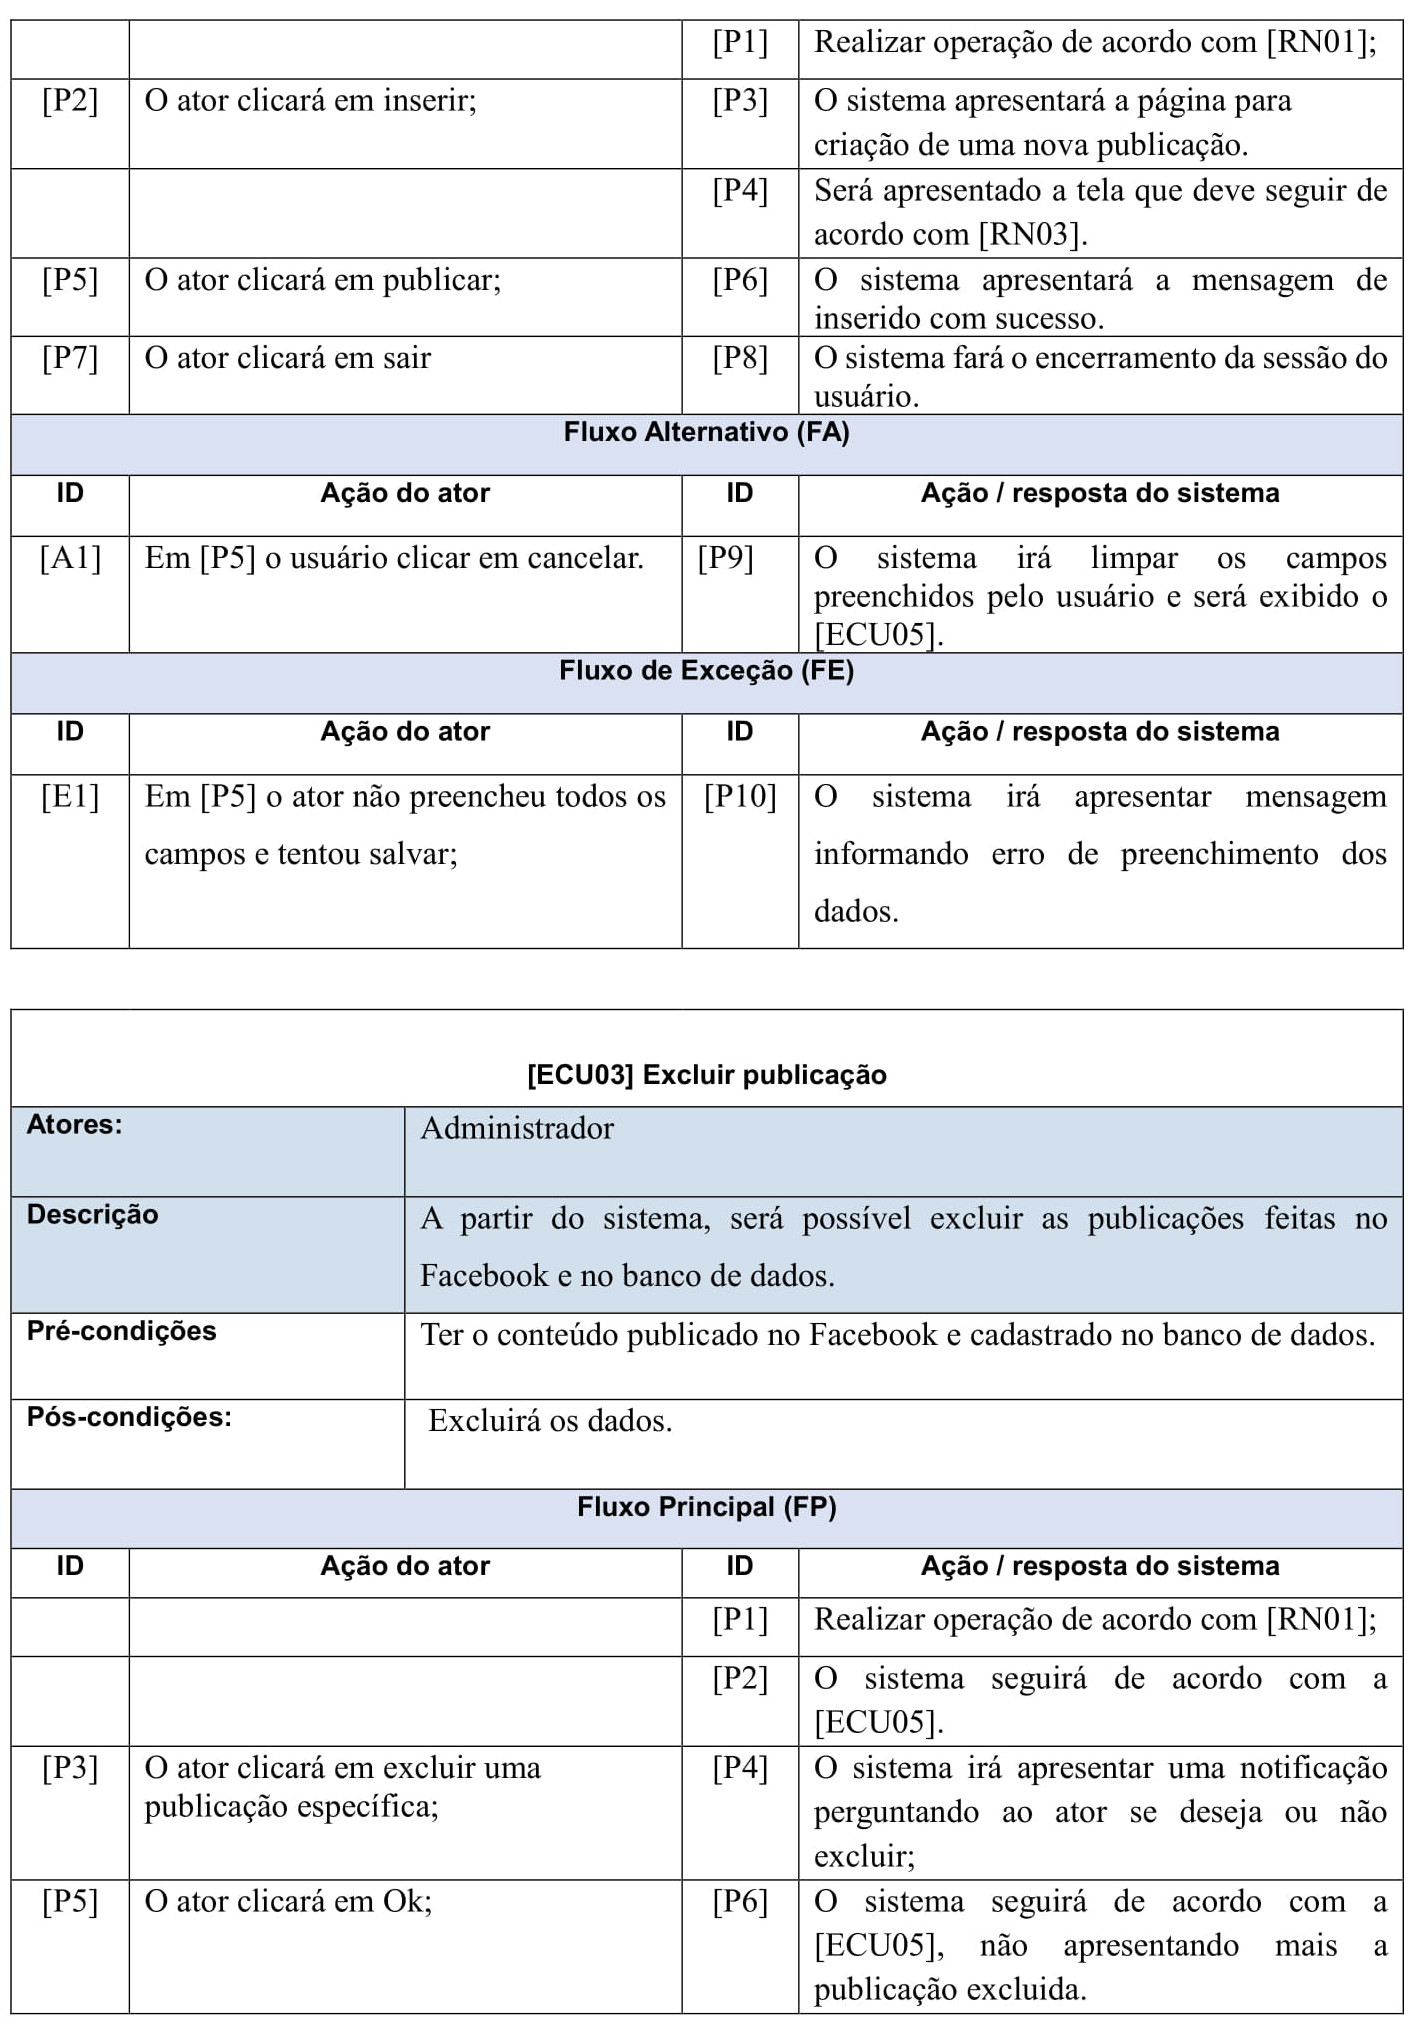
\includegraphics[width=\textwidth]{documentacao/ModeloArtefatos-07.jpg}
\end{figure}

\begin{figure}
    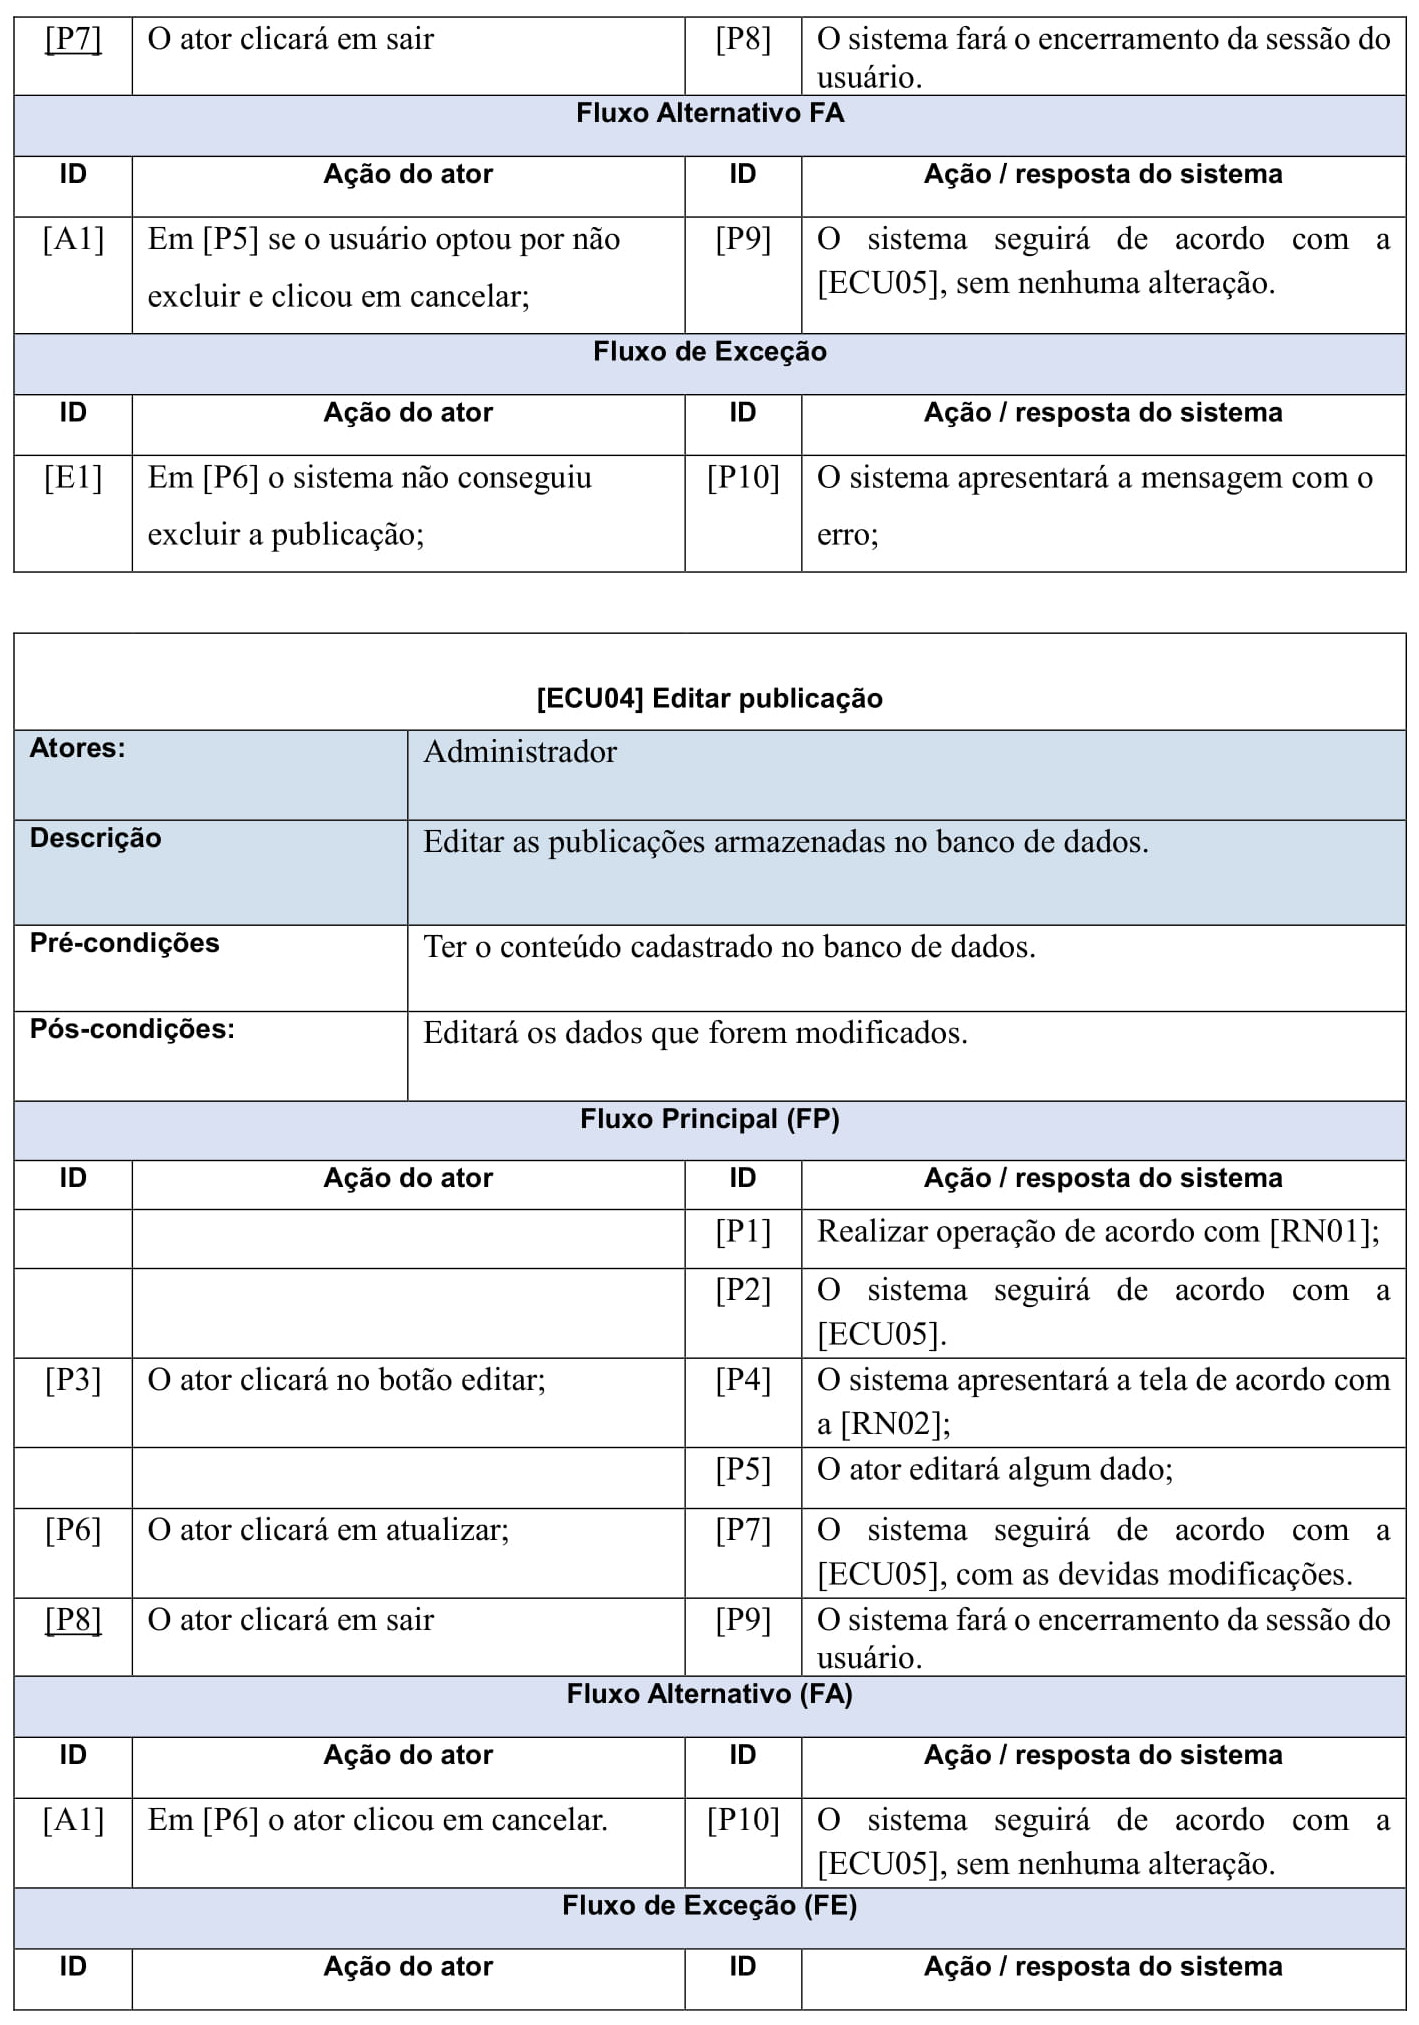
\includegraphics[width=\textwidth]{documentacao/ModeloArtefatos-08.jpg}
\end{figure}

\begin{figure}
    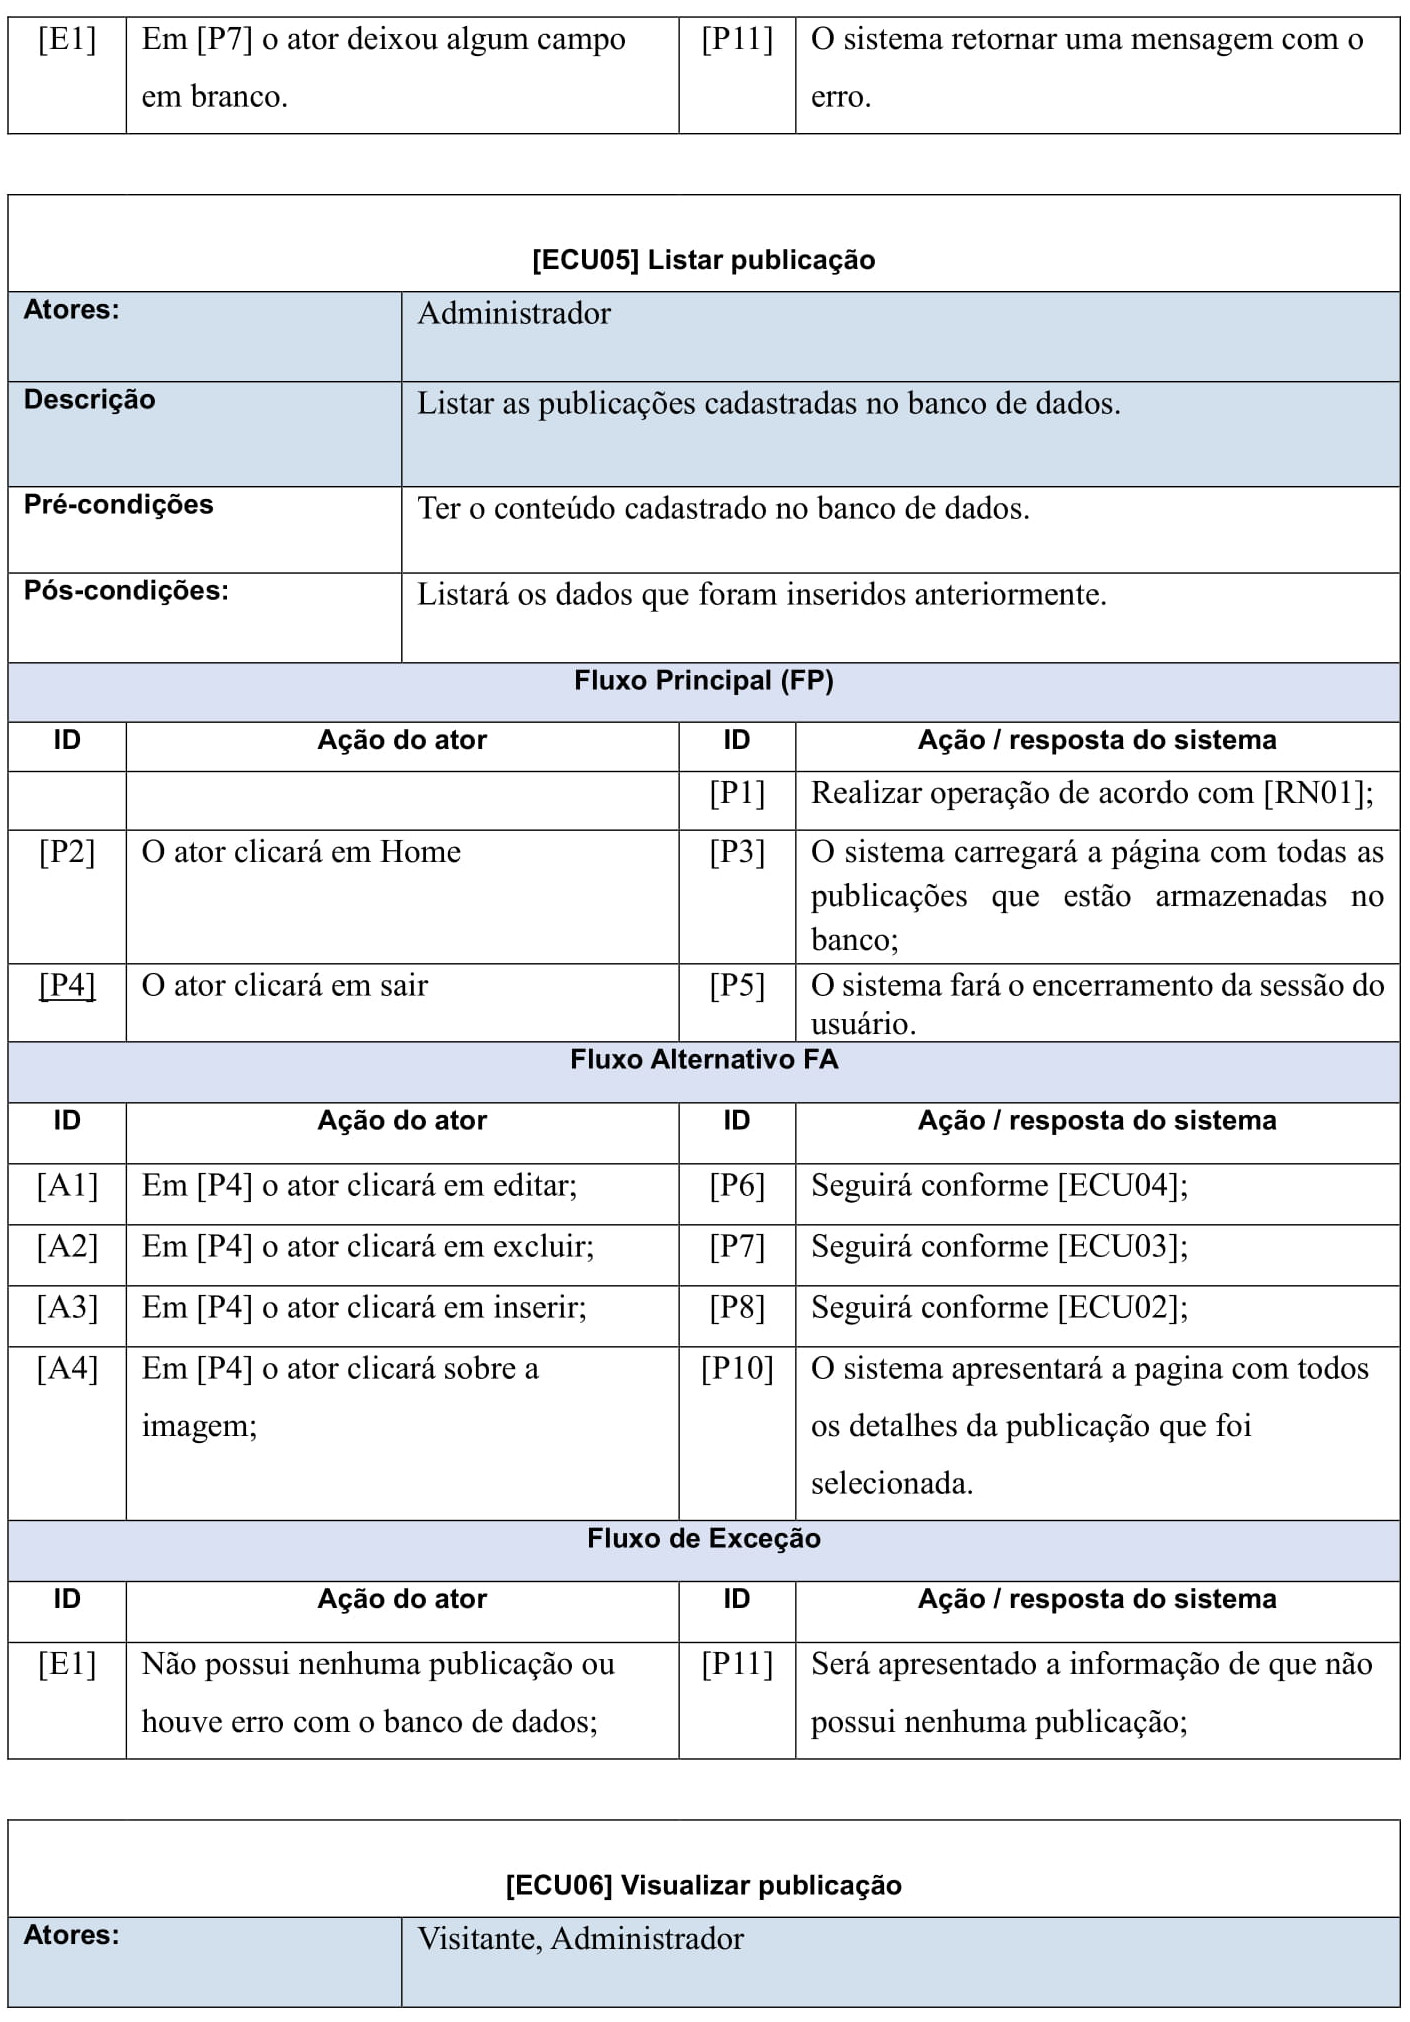
\includegraphics[width=\textwidth]{documentacao/ModeloArtefatos-09.jpg}
\end{figure}

\begin{figure}[H]
    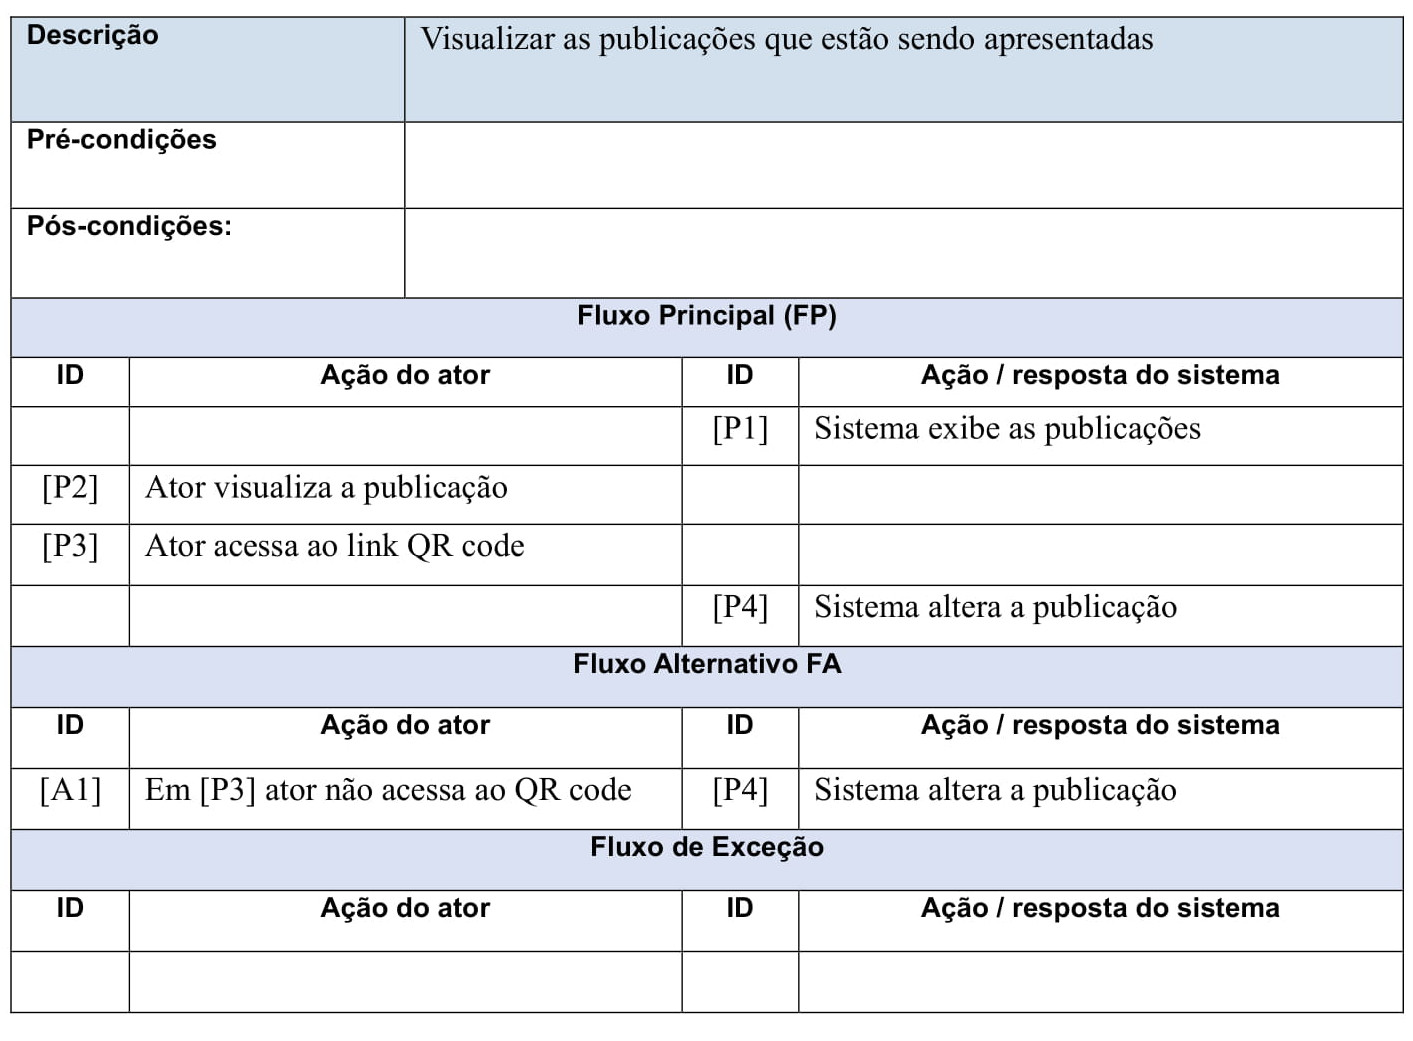
\includegraphics[width=\textwidth]{documentacao/ModeloArtefatos-10.jpg}
\end{figure}



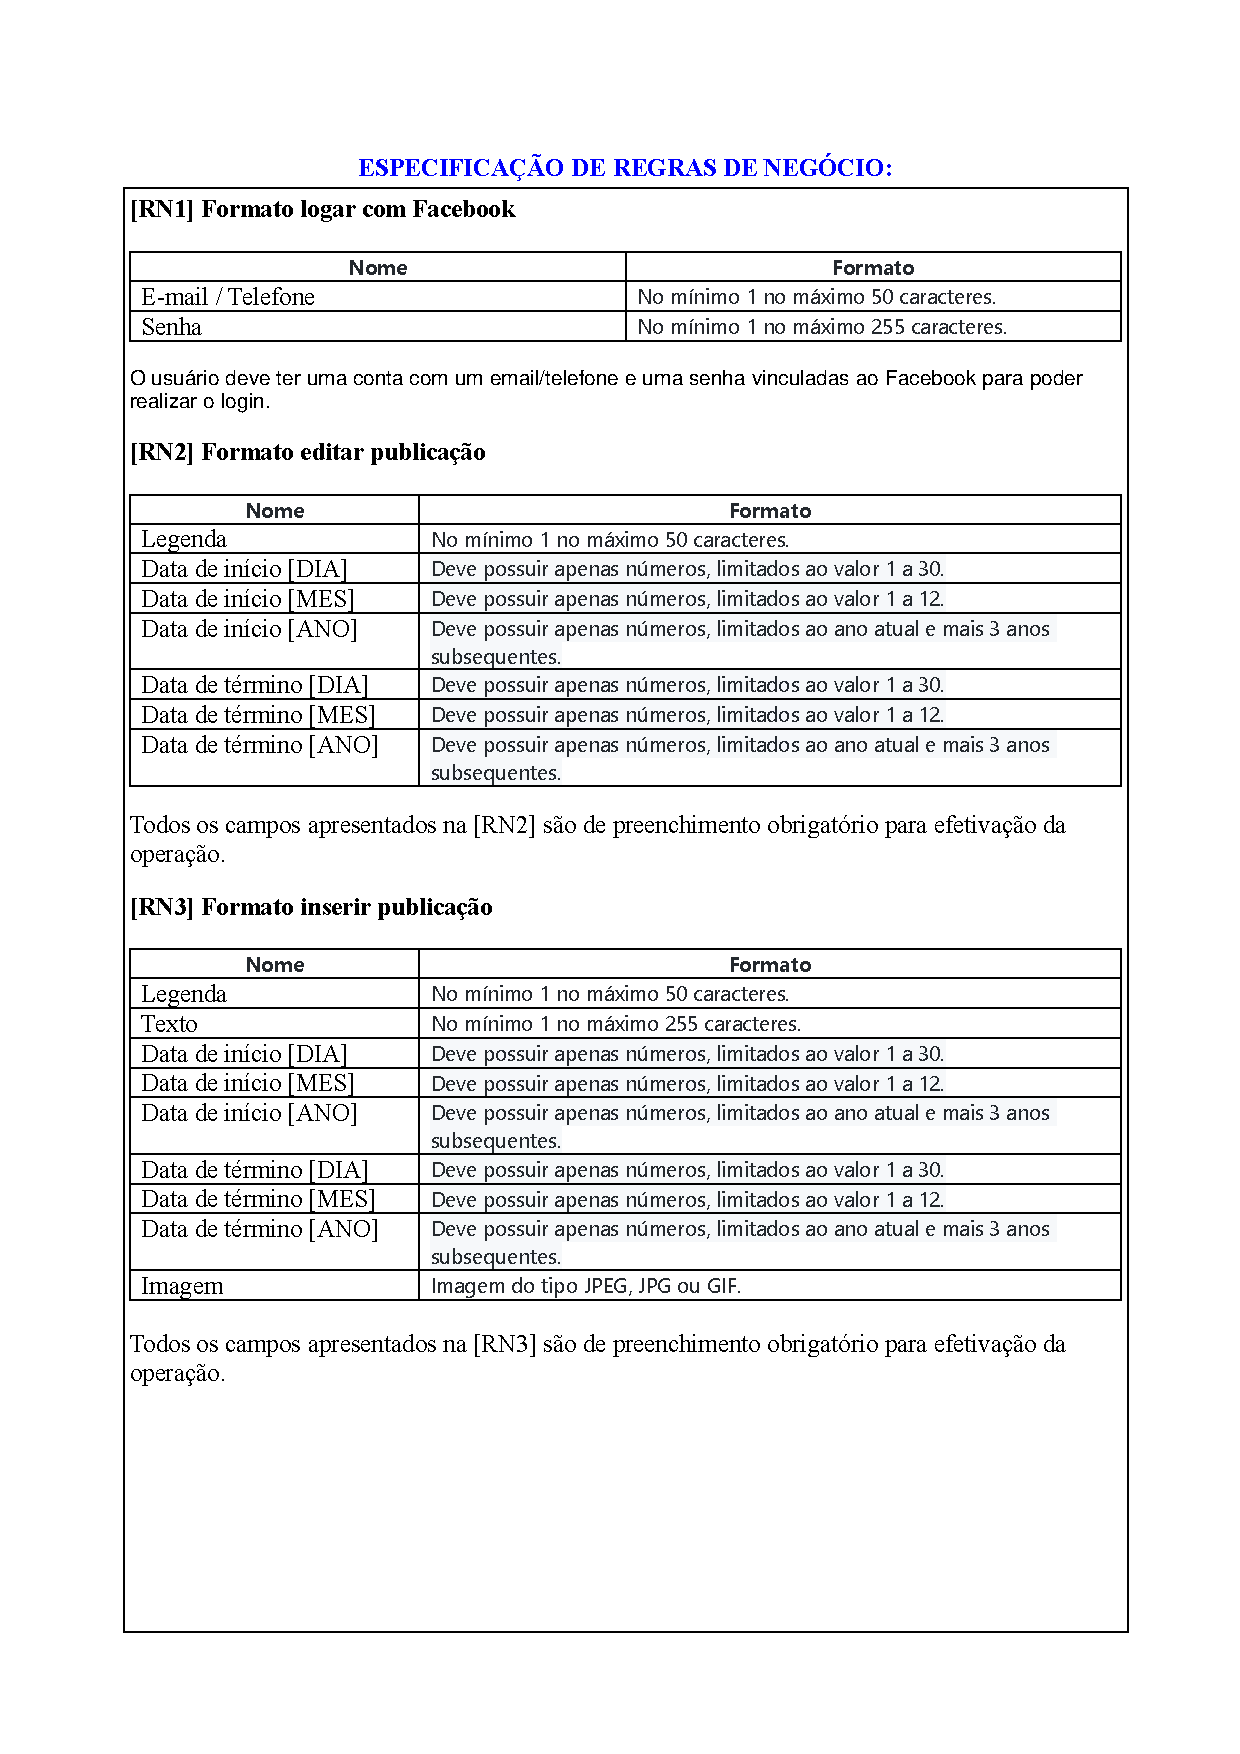
\includepdf[pages=-]{documentacao/ModeloArtefatos.pdf}

\end{document}
